% Master's thesis manuscript
% Compile from this directory with: pdflatex main.tex
% Bibliography is consolidated from references.bib using BibTeX.
\documentclass[12pt,a4paper,oneside]{report}

% Shared thesis settings. Confirm programme/institution metadata against the
% final submission requirements before submission.
\usepackage[T1]{fontenc}
\usepackage[utf8]{inputenc}
% A conventional Times-style academic serif face is used throughout the
% manuscript. The separate `times` package keeps mathematics on the standard
% Computer Modern math fonts, avoiding unavailable optional script fonts.
\usepackage{times}
\usepackage[margin=2.5cm]{geometry}
\usepackage{setspace}
\onehalfspacing
\setlength{\parindent}{0pt}
\usepackage{microtype}
\usepackage{graphicx}
\graphicspath{{figures/}}
\usepackage{pdfpages}
\usepackage{booktabs}
\usepackage{longtable}
\usepackage{tabularx}
\usepackage{array}
\usepackage{amsmath}
\usepackage{xcolor}
\usepackage{enumitem}
\usepackage{titlesec}
\usepackage{caption}
\usepackage{float}
\usepackage{etoolbox}
\usepackage[numbers,sort&compress]{natbib}
\usepackage[hidelinks]{hyperref}

% Heading hierarchy: chapter titles are deliberately prominent, with each
% lower level stepping down in size while remaining visibly distinct from the
% 12 pt body text.
% The document class supplies a 12 pt body font; one-and-a-half spacing is set
% above for readability and consistency with the submission guidance.
\titleformat{\chapter}[display]
  {\normalfont\bfseries\fontsize{18}{22}\selectfont}
  {\chaptername\ \thechapter}{0.7em}{}
\titlespacing*{\chapter}{0pt}{-8pt}{24pt}
\titleformat{\section}
  {\normalfont\bfseries\fontsize{15}{18}\selectfont}
  {\thesection}{0.8em}{}
\titleformat{\subsection}
  {\normalfont\bfseries\fontsize{13.5}{16}\selectfont}
  {\thesubsection}{0.8em}{}
\titleformat{\subsubsection}
  {\normalfont\bfseries\fontsize{12}{14.5}\selectfont}
  {\thesubsubsection}{0.8em}{}

% Captions, tables and footnotes are set at 10 pt as requested.
\DeclareCaptionFont{thesiscaption}{\fontsize{10}{12}\selectfont}
\captionsetup{font=thesiscaption,labelfont=bf}
\AtBeginEnvironment{table}{\fontsize{10}{12}\selectfont}
\AtBeginEnvironment{tabular}{\fontsize{10}{12}\selectfont}
\AtBeginEnvironment{tabularx}{\fontsize{10}{12}\selectfont}
\AtBeginEnvironment{longtable}{\fontsize{10}{12}\selectfont}
\makeatletter
\renewcommand{\footnotesize}{\@setfontsize\footnotesize{10}{12}}
\makeatother

% Keep the initial scaffold compatible with a minimal TeX installation.
% Replace these with siunitx if a full TeX distribution is used later.
\newcommand{\SI}[2]{#1~#2}
\newcommand{\micro}{\ensuremath{\mu}}
\newcommand{\metre}{m}
\newcommand{\chapref}[1]{Chapter~\ref{#1}}
\newcommand{\secref}[1]{Section~\ref{#1}}

\newcommand{\thesistitle}{Predicting Retinal Sensitivity From Optical Coherence Tomography in Usher Syndrome}
\newcommand{\authorname}{Shreeya Chandel}
\newcommand{\modulecode}{COMP0192}
\newcommand{\degreeprogramme}{MSc Artificial Intelligence for Biomedicine and Healthcare}
\newcommand{\departmentname}{University College London}
\newcommand{\submissiondate}{August 2026}
\newcommand{\publiceditiondate}{September 2026}

\hypersetup{
  pdftitle={Predicting Retinal Sensitivity From Optical Coherence Tomography in Usher Syndrome - Public Edition},
  pdfauthor={Shreeya Chandel},
  pdfsubject={Public edition of an MSc dissertation},
  pdfkeywords={OCT, microperimetry, retinal sensitivity, Usher syndrome, machine learning}
}

\newcommand{\pending}[1]{\par\noindent\fcolorbox{orange!70!black}{orange!12}{\parbox{0.92\linewidth}{\textbf{Writing prompt.} #1}}\par}
\newcommand{\resultsgate}{\textbf{Result gate:} Insert model-performance values, rankings, confidence intervals, and final figures only from the validated outputs of the self-contained master reproducibility notebook. Do not use superseded approximately 0.75~mm branch results.}
\newcommand{\resultpending}[1]{\textit{[Pending validated output: #1]}}
\newcommand{\tablepending}{\textit{TBC}}
\newcommand{\figureplaceholder}[3]{%
  \begin{figure}[htbp]
    \centering
    \fcolorbox{gray!70}{gray!10}{\parbox[c][0.22\textheight][c]{0.82\textwidth}{\centering\textbf{Figure slot}\\[0.5em]#1}}
    \caption{#2}
    \label{#3}
  \end{figure}%
}

\setlist{noitemsep,topsep=0.4em}
\setcounter{secnumdepth}{3}
\setcounter{tocdepth}{2}


\begin{document}

\pagenumbering{gobble}
\begin{titlepage}
  \centering
  \vspace*{2.5cm}
  {\Large\bfseries \modulecode\par}
  \vspace{2.5cm}
  {\Huge\bfseries \thesistitle\par}
  \vspace{2cm}
  {\Large \authorname\par}
  \vspace{0.6cm}
  {\large \degreeprogramme\par}
  \vspace{0.25cm}
  {\large \departmentname\par}
  \vfill
  {\large Submitted \submissiondate\par}
  \vspace{0.35cm}
  {\large\bfseries Public portfolio edition\par}
  {\large \publiceditiondate\par}
\end{titlepage}

\clearpage
\pagenumbering{roman}

\clearpage
\phantomsection
\begin{center}
  {\normalfont\bfseries\fontsize{18}{22}\selectfont Abstract\par}
\end{center}
\addcontentsline{toc}{chapter}{Abstract}
\begin{center}
  \begin{minipage}{0.88\textwidth}
    \setlength{\parindent}{0pt}
    \setlength{\parskip}{0pt}
    Some retinal diseases are the result of altered genes and can lead to progressive vision loss. Usher syndrome is one such condition that impacts vision and hearing simultaneously. With recent advances in gene therapy research, it has become increasingly important to measure the impacts of therapy objectively and efficiently. This project addresses this need using a use case involving patients with Usher syndrome. Two image-based data types are used. The structural type consists of optical coherence tomography (OCT) scans, which provide cross-sectional images of the eye. The second data type is microperimetry, which measures visual sensitivity at different points of the retina. Microperimetry provides a functional measurement; however, it is time-consuming and depends on patient concentration, making it difficult to repeat reliably, especially for patients with Usher syndrome who experience visual and auditory loss simultaneously. This thesis examines whether OCT can provide useful information about retinal sensitivity, potentially supporting more practical monitoring without treating imaging as a replacement for functional testing. Previous studies have demonstrated relationships between retinal structure and function in several diseases, but there is limited evidence for this approach in small and heterogeneous Usher syndrome cohorts. The study therefore develops a transparent workflow in which matched microperimetry and OCT examinations are spatially aligned, and local structural information is compared with the sensitivity measured at each retinal point. The scope of this project is narrow, with data from 22 patients and 37 recorded MAIA sensitivity points per accepted eye-visit. Model performance is assessed using complementary measures of prediction error, agreement and calibration, with uncertainty estimated at patient level. The resulting framework provides a reproducible investigation into retinal structure--function relationships in an Usher syndrome cohort and analyses what functional predictions can reasonably be inferred from OCT structure.

  \end{minipage}
\end{center}

\clearpage
\phantomsection
\begin{center}
  {\normalfont\bfseries\fontsize{18}{22}\selectfont Acknowledgements\par}
\end{center}
\addcontentsline{toc}{chapter}{Acknowledgements}
\begin{center}
  \begin{minipage}{0.88\textwidth}
    \setlength{\parindent}{0pt}
    \setlength{\parskip}{0pt}
    I would like to express my sincere gratitude to Dr Adam Dubis for his supervision, guidance and feedback throughout this project. I also thank the clinical, research and data-governance teams who collected, curated and prepared the retinal imaging and microperimetry data used in this study, as well as my colleagues, friends and family for their practical and personal support during the project.

  \end{minipage}
\end{center}

\clearpage
\phantomsection
\begin{center}
  {\normalfont\bfseries\fontsize{18}{22}\selectfont Declaration\par}
\end{center}
\addcontentsline{toc}{chapter}{Declaration}
I, Shreeya Chandel, confirm that the work presented in this thesis is my own. Where information, ideas, data, code, figures or other material have been derived from other sources, I have indicated this through appropriate citation, acknowledgement or attribution.

I have used all third-party material included in this thesis in accordance with the relevant permission, licence, data-governance or quotation requirements. I accept responsibility for the analyses, interpretations and conclusions presented, and I have checked the submitted content and its supporting sources.

I used generative artificial-intelligence tools during preparation of the manuscript for limited assistance with LaTeX formatting, language editing and organisation of material. I retained responsibility for the substantive argument, analysis, interpretation, references and final wording, and reviewed and verified all assisted material.


\begingroup
\singlespacing
\tableofcontents
\endgroup
\listoffigures
\listoftables

\clearpage
\pagenumbering{arabic}

\chapter{Introduction}
\label{chap:introduction}

\section{Study overview}

Usher syndrome is an inherited retinal degenerative condition that combines hearing impairment with vision loss \cite{Whatley2020,Toualbi2020}. Optical coherence tomography (OCT) is an objective imaging scan of retinal structure, whereas microperimetry measures a patient's functional vision: the sensitivity of different retinal points to visual stimuli \cite{Langlo2025,Pfau2021Microperimetry}. This thesis examines a focused structure--function question: whether local information from OCT can be used to estimate the retinal sensitivity measured at the corresponding location by fundus-controlled microperimetry, within an Usher syndrome cohort.

The prediction target is intentionally narrow. At each tested retinal location, the target is to obtain information that permits an estimate for a point not used to train the model, after allowing for variation due to location or average sensitivity. The study aims to investigate the information contained in OCT examinations for research, future monitoring and assessing gene-therapy efficacy, rather than to establish OCT as a replacement for functional testing.

The available dataset contains paired OCT and MAIA microperimetry examinations from people with Usher syndrome. Each microperimetry result comprises 38 sensitivity locations per eye, while the OCT volume contains detailed structural information across the retina. The central methodological task is therefore to establish a defensible spatial correspondence between the two modalities and then evaluate whether the OCT information assigned to each point improves prediction over simple alternatives.

\section{Aim and objectives}

\textbf{Overall aim.} To determine whether, and to what extent, OCT-derived information can predict pointwise retinal sensitivity in a cohort of participants with Usher syndrome, and to evaluate relevant metrics and limits of those predictions.

\textbf{Objectives.}
\begin{enumerate}
  \item Critically synthesise the biological, clinical and computational evidence that motivates a structure--function prediction study in Usher syndrome.
  \item Construct and quality-control spatially matched MAIA--OCT/SLO observations, including registration, point-to-B-scan mapping and point-level pooling within the functional footprint.
  \item Test whether the primary full-cohort OCT representation improves prediction beyond null, fixed-reference and retinal-location baselines under participant-grouped nested validation.
  \item Evaluate, in the boundary-available secondary cohort, whether B0--B4 source-mapped structural features and boundary-aligned image representations add predictive information.
  \item Report complementary measures of error, agreement, calibration and participant-level uncertainty, including the implications of the microperimetry device floor.
  \item Define the evidential boundary of the findings and the requirements for external, longitudinal or clinical validation.
\end{enumerate}

\section{Research questions}

\begin{enumerate}[label=\textbf{RQ\arabic*.},leftmargin=*]
  \item Retinal sensitivity reflects both a point's position in the retinal field and the condition of the local tissue. Geometric and location features may appear predictive without describing retinal biology, while the human-verified boundary features are available only for a smaller cohort. To what extent does biological context from OCT-derived image and boundary features add predictive information beyond geometric context and retinal-location features?

  \item A pointwise structure--function analysis requires each MAIA sensitivity location to be matched to the corresponding area of the OCT volume. MAIA and OCT/SLO examinations use different coordinate systems, and registration or point-to-scan errors can associate a sensitivity value with unrelated retinal tissue. Can the two examinations be registered and quality-controlled so that each MAIA point is assigned to a defensible local OCT region for subsequent modelling?

  \item Existing studies suggest that retinal function can be estimated from structural imaging in several retinal diseases. Their diseases, endpoints, sample sizes, representations and validation procedures differ from those of the present small and heterogeneous Usher syndrome cohort. Can modelling strategies supported by existing structure--function studies provide useful participant-held-out predictions when adapted to the present cohort?

  \item Image-derived representations may capture structural information that is not available from simple features. The available clinical cohort is limited, and source-mapped boundary features are available only for a subset of the observations. Given that large image models can overfit limited clinical data, can a frozen retinal foundation-model representation and constrained regression models make useful predictions for participants not used during training, and what additional information is provided by source-mapped boundary features where these are available?

  \item A more objective estimate of local retinal function could support the study of retinal structure--function relationships. The cohort is small, and points, eyes and visits from the same participant are correlated. Given the need for a more objective estimate of local retinal function, can spatially aligned OCT information improve the prediction of pointwise MAIA sensitivity beyond non-imaging baselines, despite the small cohort and the correlation between points, eyes and visits from the same participant?
\end{enumerate}

\section{Thesis outline}

Chapter~\ref{chap:introduction} introduces the study, its aim, objectives and research questions. Chapter~\ref{chap:background} presents the biological and clinical context, reviews previous retinal structure--function studies and explains how the evidence informed the project. Chapter~\ref{chap:methods} describes the data, registration, pointwise OCT sampling, primary and secondary analyses, modelling strategy and participant-grouped evaluation. Chapter~\ref{chap:results} reports the cohort, registration outcomes and predictive results for both analyses. Chapter~\ref{chap:discussion} interprets the findings in relation to the research questions and existing evidence, while considering their reliability and clinical meaning. Chapter~\ref{chap:conclusion} summarises the main contribution of the thesis, and Chapter~\ref{chap:future-work} identifies the methodological and clinical work needed before the approach can be evaluated beyond the present cohort.

\chapter{Background and Literature Review}
\label{chap:background}

This chapter establishes the biological and clinical basis of the project before reviewing the evidence for estimating retinal function from structural imaging. The review concentrates on work that directly informed the present study: structure--function relationships in Usher syndrome and inherited retinal degeneration, prediction of retinal sensitivity in related retinal diseases, and methodological decisions that become important when the number of participants is small.

\section{Review method}

The structured literature review covered publications from 2014 to 2026. Five sources were selected from an initial list of thirteen because they provided complementary coverage of clinical ophthalmology and computational imaging: PubMed, Embase through Ovid, Scopus, IEEE Xplore and the ACM Digital Library. Search terms were organised into three groups. The disease group included Usher syndrome, \textit{USH2A}, retinitis pigmentosa and inherited retinal degeneration; the measurement group included OCT, microperimetry, retinal sensitivity, fundus autofluorescence and structure--function; and the methods group included machine learning, deep learning, regression, transfer learning and common evaluation measures. Separate searches for Macular Telangiectasia and age-related macular degeneration were used to identify the closest methodological comparators, and backward citation searching from the RUSH2A and ReSensNet papers was used to find earlier work that did not use current machine-learning terminology.

The review recorded 785 papers within the combined search scope, from which 14 studies were retained after screening. The eligibility criteria applied during screening are summarised in Table~\ref{tab:review-criteria}.

\begin{table}[H]
\centering
\caption{Inclusion and exclusion criteria used in the structured literature review.}
\label{tab:review-criteria}
\begin{tabularx}{\textwidth}{@{}>{\raggedright\arraybackslash}p{0.16\textwidth}>{\raggedright\arraybackslash}X@{}}
\toprule
Decision & Criterion \\
\midrule
Inclusion & Studies of retinal structure--function relationships in Usher syndrome, retinitis pigmentosa or inherited retinal degeneration, together with transferable retinal comparators including Macular Telangiectasia, age-related macular degeneration, geographic atrophy and diabetic macular oedema. \\
Inclusion & Studies using OCT, fundus autofluorescence or related structural retinal imaging to report quantitative functional outcomes, biomarker correlations or sensitivity-related endpoints. \\
Inclusion & Machine-learning, deep-learning or statistical studies reporting quantitative performance, and foundational clinical studies that informed model design, endpoint selection or characterisation of the target dataset. \\
Inclusion & Methodological studies relevant to small retinal-imaging datasets, including transfer learning, self-supervised learning, segmentation and measurement-reliability analysis. \\
Exclusion & Reviews, systematic reviews, opinion articles or conference abstracts without full peer-reviewed methods. \\
Exclusion & Studies limited to retinal conditions outside the defined scope, such as glaucoma or non-macular diabetic retinopathy, without a transferable structure--function method. \\
Exclusion & Studies without quantitative outcomes, or with insufficient methodological detail for meaningful quality assessment. \\
\bottomrule
\end{tabularx}
\end{table}

The retained papers were assessed for study design, sample selection, imaging and registration, validation, reported metrics, ethics and generalisability.

\section{Biological and clinical context}

\subsection{Usher syndrome and retinal degeneration}

Usher syndrome is a genetically diverse, usually autosomal-recessive condition that combines sensorineural hearing loss with retinitis pigmentosa; vestibular function may also be affected \cite{Mathur2015,Whatley2020}. Variants in \textit{USH2A} are an important cause of Usher syndrome type 2 and may also cause non-syndromic autosomal-recessive retinitis pigmentosa \cite{Toualbi2020,Lad2022}.

Vision depends on rod and cone photoreceptors converting light into neural signals. Rods support low-light and peripheral vision, whereas cones are more important for detailed central and colour vision \cite{Salesse2017}. Retinitis pigmentosa often affects rods first. Night vision and the peripheral visual field may therefore worsen while central vision remains useful.

Usher proteins help to maintain photoreceptor structure and the movement of molecules between the inner and outer segments. When these processes are disrupted, photoreceptor function and structure can progressively deteriorate \cite{Whatley2020,Mathur2015}. The uneven pattern of degeneration also explains why central visual acuity alone provides an incomplete account of vision. Measurements taken across different retinal locations are needed to describe both the remaining structure and the corresponding local function.

\subsection{OCT markers of remaining photoreceptor structure}

OCT uses low-coherence interferometry to form non-invasive depth profiles of tissue. A single axial reflectivity profile is an A-scan; adjacent A-scans form a cross-sectional B-scan, and a set of neighbouring B-scans forms a retinal volume \cite{Huang1991,Langlo2025}. The resulting image is an optical representation rather than a histological section, but it permits retinal layers and reflective bands to be examined in vivo.

The outer retina contains several features relevant to inherited degeneration. The ONL contains the photoreceptor cell bodies, while the ellipsoid zone (EZ) is a reflective OCT band associated with the photoreceptor inner-segment region. The term ``zone'' is deliberately cautious because the precise anatomical sources of some OCT bands are not completely settled \cite{Staurenghi2014,Tao2016}. Continuity or extent of the EZ and preservation of the ONL can therefore indicate remaining photoreceptor structure, but a visible feature is not itself a measurement of vision. The boundary values supplied for the secondary analysis are consequently retained as the neutral labels B0--B4; anatomical names are not assigned without independent verification of their source definitions.

\section{OCT and microperimetry as complementary measurements}

Fundus-controlled perimetry, commonly called microperimetry, measures light sensitivity at defined retinal locations while imaging and tracking the fundus. Sensitivity is reported in decibels, so the resulting map describes local function that may not be apparent from a central acuity measurement \cite{Pfau2021Microperimetry}. Its spatial resolution is particularly useful in inherited retinal degeneration, but the result remains dependent on the participant seeing and responding to the stimulus. Fixation, attention, fatigue, learning and disease severity can all influence repeated measurements.

This uncertainty is greater for individual locations than for an average across the test grid. In the REPEAT study of retinitis pigmentosa, the reported pointwise coefficient of repeatability was approximately 8.6--10.2 dB, whereas repeatability for mean sensitivity was approximately 0.9--2.4 dB \cite{Karuntu2025}. These values cannot be transferred directly to every device, protocol or cohort, but they show why a pointwise prediction error should not be interpreted in the same way as an error for an eye-level mean. Values at the device floor also require separate attention because different levels of severe loss can be recorded at the same lower limit.

OCT and microperimetry thus provide different information: OCT records structure objectively and rapidly, whereas microperimetry records a psychophysical response. To analyse their relationship, a functional test point must first be registered to the corresponding retinal position in the OCT reference image. An incorrect transform, or the use of an OCT region much larger than the stimulus location, may assign unrelated structure to the same sensitivity label. Spatial registration and local sampling are therefore part of the scientific validity of a structure--function model, rather than simply preprocessing details.

\section{Disease-specific structure--function evidence}

The strongest direct evidence came from studies of \textit{USH2A}-related degeneration. In the RUSH2A natural-history cohort, Lad et al. analysed 127 participants, including 80 with Usher syndrome type 2 and 47 with non-syndromic autosomal-recessive retinitis pigmentosa; 93 participants also had microperimetry \cite{Lad2022}. Longer disease duration was associated with a smaller intact EZ area and lower mean sensitivity, while larger EZ area and central retinal thickness were associated with better function. The review recorded a correlation of $r=0.68$ between EZ area and mean sensitivity. This provides disease-specific evidence that preserved structure and function are related, but it remains a cohort-level association rather than a test of pointwise prediction in unseen participants.

Gill et al. reported that EZ width explained a substantial proportion of variation in visual acuity in a smaller \textit{USH2A} cohort ($R^2=0.717$), again supporting the importance of outer-retinal preservation while using a different functional outcome \cite{Gill2022}. Charng et al. examined edge-of-scotoma sensitivity as a possible longitudinal endpoint and found it more responsive to change than several broader measures in a small cohort \cite{Charng2020}. Together, these studies justify examining local structural information, but they do not establish that an OCT model will estimate MAIA sensitivity accurately, nor that a prediction can replace the functional test.

\section{Prediction studies in related retinal diseases}

\subsection{Interpretable statistical models}

Studies in age-related macular degeneration provide useful methodological precedents because they aligned local OCT or fundus features with pointwise sensitivity. Wu et al. used graded microstructural features and stepwise regression, reporting a strong relationship between predicted and measured sensitivity, although the expert grading limits scalability \cite{Wu2014}. Pfau et al. used random forests with OCT thickness, intensity and fundus features in geographic atrophy. Under patient-wise leave-one-out validation, their imaging-only model had an MAE of 4.64 dB, which improved to 2.89 dB when limited patient-specific calibration data were included; ONL-related features were among the most important predictors \cite{Pfau2020}. A related study in neovascular age-related macular degeneration reported a calibrated MAE of 2.80 dB \cite{vonderEmde2019}. These results demonstrate that relatively small, structured models can extract interpretable information, but patient-specific calibration changes the question from prediction for a wholly unseen participant.

\subsection{Deep learning and representation transfer}

Kihara et al. trained a convolutional network on local OCT patches in Macular Telangiectasia type 2 and reported an MAE of 3.36 dB and a correlation of 0.78 \cite{Kihara2019}. The difference between its lower training error and higher test error also illustrates the overfitting risk created by a high-capacity model and a small number of patients. In retinitis pigmentosa, Le et al. reported $R^2=0.79$ using a wavelet-based deep network, while Nagasato et al. used an ensemble of pretrained fundus-image networks and obtained rank correlations of approximately 0.68--0.70 for visual-field summaries \cite{Le2024,Ding2023}. These studies support the feasibility of image-based functional estimation, but they use different diseases, inputs, endpoints and validation splits, so their headline values are not direct benchmarks for pointwise MAIA prediction in Usher syndrome.

Pretraining offers one response to limited labelled data. Self-supervised retinal training has shown that useful image representations can be learned from unlabelled OCT volumes, and RETFound demonstrated that a retinal foundation model could transfer to several disease-detection tasks \cite{Gholami2024,Zhou2023RETFound}. Transfer is not guaranteed, however. Loo et al. found that an EZ segmentation model transferred poorly from Macular Telangiectasia to \textit{USH2A} scans until it was retrained on disease-specific data \cite{Loo2022}. A frozen RETFound encoder is therefore a reasonable constrained representation for this thesis, but its success in classification does not establish its value for local regression.

\section{Validation, evaluation and critical gap}

The reviewed evidence was difficult to compare because studies differed in the unit of prediction, use of calibration, outcome range and validation design. The distinction between retinal points and independent participants is especially important. Many points, two eyes and repeated visits can come from one person; a random point-level split would allow closely related observations to appear in both training and test sets and could produce an optimistic estimate of generalisation. Patient-wise splitting in the stronger small-cohort studies informed the participant-grouped validation used here.

No single evaluation measure answers the whole question. MAE expresses average absolute error in the original dB scale, while RMSE gives greater weight to large errors. Correlation measures whether observations and predictions vary together but can remain high when predictions are systematically biased. $R^2$ compares performance with a mean prediction and can be negative in held-out data. Calibration and Bland--Altman analysis add information about systematic under- or over-prediction and agreement across the sensitivity range. These measures need to be interpreted together and with participant-level uncertainty.

The literature therefore supports the biological plausibility of local structure--function modelling and shows that retinal images can contain predictive information. It does not provide direct evidence that OCT can predict pointwise MAIA sensitivity in Usher syndrome under participant-held-out validation. This gap shaped the present study: registration was checked explicitly; observations were reduced to one representation per MAIA point; model complexity was constrained; non-imaging baselines were included; folds were grouped by participant; and error, agreement, calibration and uncertainty were reported together. The full-cohort image analysis addresses the main question, while the smaller boundary-available analysis provides a separate, more interpretable examination of local structural features. Chapter~\ref{chap:methods} describes how these decisions were implemented.

\begin{table}[htbp]
\centering
\caption{Selected studies from the literature review and the design lesson carried into this thesis.}
\label{tab:literature-metrics}
\begin{tabularx}{\textwidth}{@{}>{\raggedright\arraybackslash}p{0.20\textwidth}>{\raggedright\arraybackslash}p{0.21\textwidth}>{\raggedright\arraybackslash}p{0.20\textwidth}>{\raggedright\arraybackslash}X@{}}
\toprule
Study and disease & Target and approach & Validation/metric reported & Critical relevance to the present study \\
\midrule
Lad et al.; Gill et al. (USH2A) & EZ area/width with statistical association or linear regression & $r=0.68$; $R^2=0.717$; no held-out prediction & Establishes disease-specific plausibility, but not unseen-participant pointwise prediction. \\
Kihara et al. (MacTel2) & CNN from local OCT patches & MAE $=3.36$ dB; patient-level split & Demonstrates feasibility while exposing a large train--test gap and high-capacity overfitting risk. \\
Pfau et al.; von der Emde et al. (GA/nAMD) & Random forest from layer and intensity features & Patient-wise LOO; MAE $=2.89$ and $2.80$ dB with calibration & Provides interpretable small-sample baselines and supports reporting against a repeatability reference. \\
Le et al.; Nagasato et al. (RP) & Deep OCT or fundus representations & $R^2=0.79$ or rank correlations; single/external split variants & Shows transferability of the idea, but endpoints and metrics are not directly comparable with local MAIA sensitivity. \\
Karuntu et al. (RP) & Test--retest reliability of microperimetry & Pointwise CoR $\approx8.6$--$10.2$ dB; mean-sensitivity CoR $<2.5$ dB & Defines the measurement context within which pointwise prediction error should be interpreted. \\
This thesis & Registered local OCT to pointwise MAIA sensitivity & Participant-grouped nested validation; MAE, RMSE, agreement, calibration and bootstrap uncertainty & Tests whether the reported structure--function signal persists without participant or patch leakage. \\
\bottomrule
\end{tabularx}
\end{table}

\chapter{Methodology}
\label{chap:methods}

% -----------------------------------------------------------------------
\section{Study design and analytical principles}
\label{sec:design}

The thesis was designed as an internally validated study of spatially matched OCT and MAIA microperimetry examinations from patients with Usher syndrome.

The project was guided by the following principles:

\begin{enumerate}
  \item \textbf{Pointwise regression endpoint.} The task was treated as supervised, instance-level regression. Each instance was a numbered MAIA Point 1--37, and the primary endpoint was the continuous retinal sensitivity measured at that point in decibels (dB).
  \item \textbf{One functional point as one observation.} A-scans and neighbouring B-scans describing the same MAIA point were combined into one point-level representation.
  \item \textbf{Outcome-independent representation construction.} The structural representations were made without using sensitivity values. Sensitivity was joined only after the representation had been fixed.
  \item \textbf{Participant-level generalisation.} Several points, eyes and visits could come from one participant. Validation was therefore grouped by participant, which prevented data leakage between the training and held-out sets.
\end{enumerate}

The work was divided into two planned analyses. The \emph{primary} analysis retained all eligible point-level observations and used fixed location and image-derived OCT representations. The \emph{secondary} analysis used the smaller subset with human-verified boundary features. This made comparison of interpretable local structural features with boundary-aligned image representations possible. Results are reported separately for each cohort.

For the purpose of this thesis, the workflow can be understood as six high-level analytical stages, as highlighted in Figure~\ref{fig:method-workflow}.

\begin{figure}[H]
  \centering
  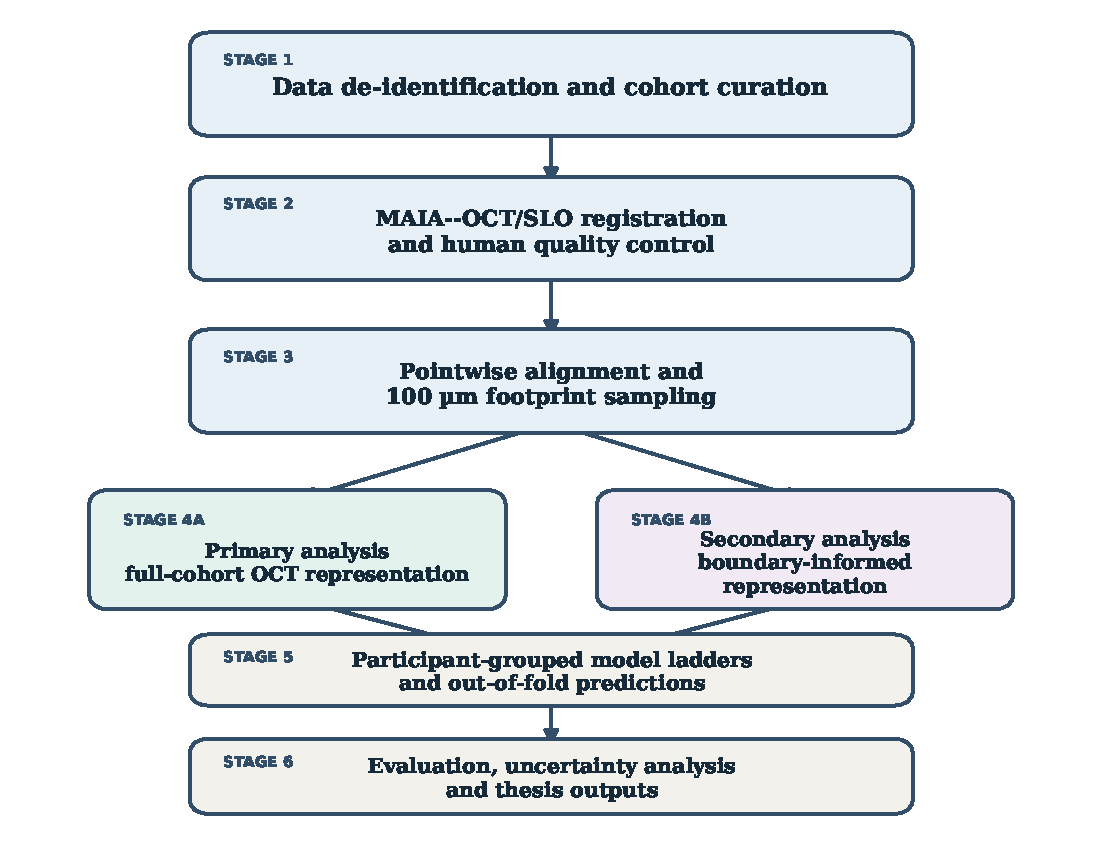
\includegraphics[width=0.92\textwidth,height=0.50\textheight,keepaspectratio]{figure_methodology_workflow.pdf}
  \caption{High-level analytical workflow. Following data preparation, registration and pointwise alignment, the workflow separates into the primary full-cohort image analysis and the secondary boundary-informed analysis. The two branches are then evaluated using participant-grouped model ladders and out-of-fold predictions.}
  \label{fig:method-workflow}
\end{figure}

% -----------------------------------------------------------------------
\section{Data sources, cohort and outcome}
\label{sec:cohort}

The data were obtained from retinal imaging and microperimetry examinations collected from patients with Usher syndrome. Each MAIA examination provided a fundus image showing the test grid and a measurement of retinal sensitivity in decibels (dB) at each test location. The corresponding OCT examination provided a volume of cross-sectional retinal B-scans, an associated scanning laser ophthalmoscopy (SLO) image and the spatial information needed to locate the scans within the fundus image. Together, these examinations provided a functional measurement from MAIA and a structural measurement from OCT for the same eye and visit.

Before analysis, the source records were de-identified and organised using study-specific patient, eye and visit labels. The usable analysis data consisted of the MAIA sensitivity values and fundus images, OCT volumes and SLO images, scan geometry, and the saved registration and quality-control records. The de-identification process allowed the data to be analysed at patient and eye-visit level without including direct patient identifiers in the working dataset.

Seventy-nine candidate same-visit eye pairs from 23 patients were identified. An eye-visit was included in the primary cohort when it contained a usable MAIA examination, matched OCT volume and SLO image, and an approved MAIA--OCT/SLO registration. One eye-visit was excluded following review because the spatial correspondence between the MAIA test locations and OCT volume was not sufficiently reliable.

The final primary cohort included 22 patients, 78 accepted eye-visits and 2,886 pointwise observations. Each eye-visit contributed the 37 numbered MAIA Points 1--37. Sensitivity was analysed as a continuous outcome, including observed $-1$~dB values at the device floor.

\begin{table}[htbp]
\centering
\caption{Composition of the primary and secondary analysis cohorts.}
\label{tab:cohort}
\begin{tabularx}{\textwidth}{Xrr}
\toprule
Item & Primary cohort & Secondary cohort \\
\midrule
Patients & 22 & 22 \\
Accepted eye-visits & 78 & 50 \\
Baseline / year-one eye-visits & 41 / 37 & 13 / 37 \\
Pointwise observations (MAIA Points 1--37) & 2,886 & 1,850 \\
Points per accepted eye-visit & 37 & 37 \\
Sensitivity floor ($-1$~dB) observations & 533 & 278 \\
\bottomrule
\end{tabularx}
\end{table}

The secondary cohort was limited to eye-visits with source-mapped, human-verified B0--B4 boundary information that could be matched to the accepted OCT volume and passed structural, mapping and placement checks. Fifty eye-visits met these criteria, giving the same 22 patients and 1,850 pointwise observations.

% -----------------------------------------------------------------------
\section{MAIA--OCT/SLO registration and quality control}
\label{sec:registration}

\subsection{Automatic transform estimation}

The MAIA fundus image was aligned to the corresponding OCT/SLO image. Both images were standardised to a common $512\times512$ display grid for registration. They were then processed to reduce broad illumination differences and emphasise vessel-like dark features. Image correlation was used to estimate the alignment.

Several starting positions were tested because the MAIA and OCT/SLO images can have different fields of view. Similarity registration was run at five scales (0.70, 0.80, 0.90, 1.00 and 1.10) and three rotation angles ($-6^{\circ}$, $0^{\circ}$ and $+6^{\circ}$), giving fifteen starting points for each eye-visit. Each run used image correlation, linear interpolation and a three-level image pyramid. The candidate with the best final metric was refined using an affine transform. The resulting transform was checked to ensure that it was geometrically plausible. Registration was implemented with SimpleITK \citep{Langlo2025}, which provides an established framework for multi-resolution image registration and applying transformations between images acquired using different modalities. The automatic registration provided a candidate alignment for human review, which determined whether the alignment was accepted.

\subsection{Human visual quality control and final use}

Each transform was saved with its warp images, overlays, transform files and registration metadata. The overlays were reviewed for vessel alignment, image doubling and anatomical plausibility. The accepted transform for each eye-visit was then recorded as a governed input. Borderline cases retained their review status in the provenance record. Eye-visits without acceptable spatial correspondence were excluded.

This combination of automatic registration and visual review was important because a transform can have a good global image score while still placing a local MAIA point in the wrong retinal position. Similarly, a globally acceptable transform does not show which B-scan or A-scan should represent an individual functional point. That question was addressed by the geometric mapping described in Section~\ref{sec:footprint}.

\begin{figure}[htbp]
  \centering
  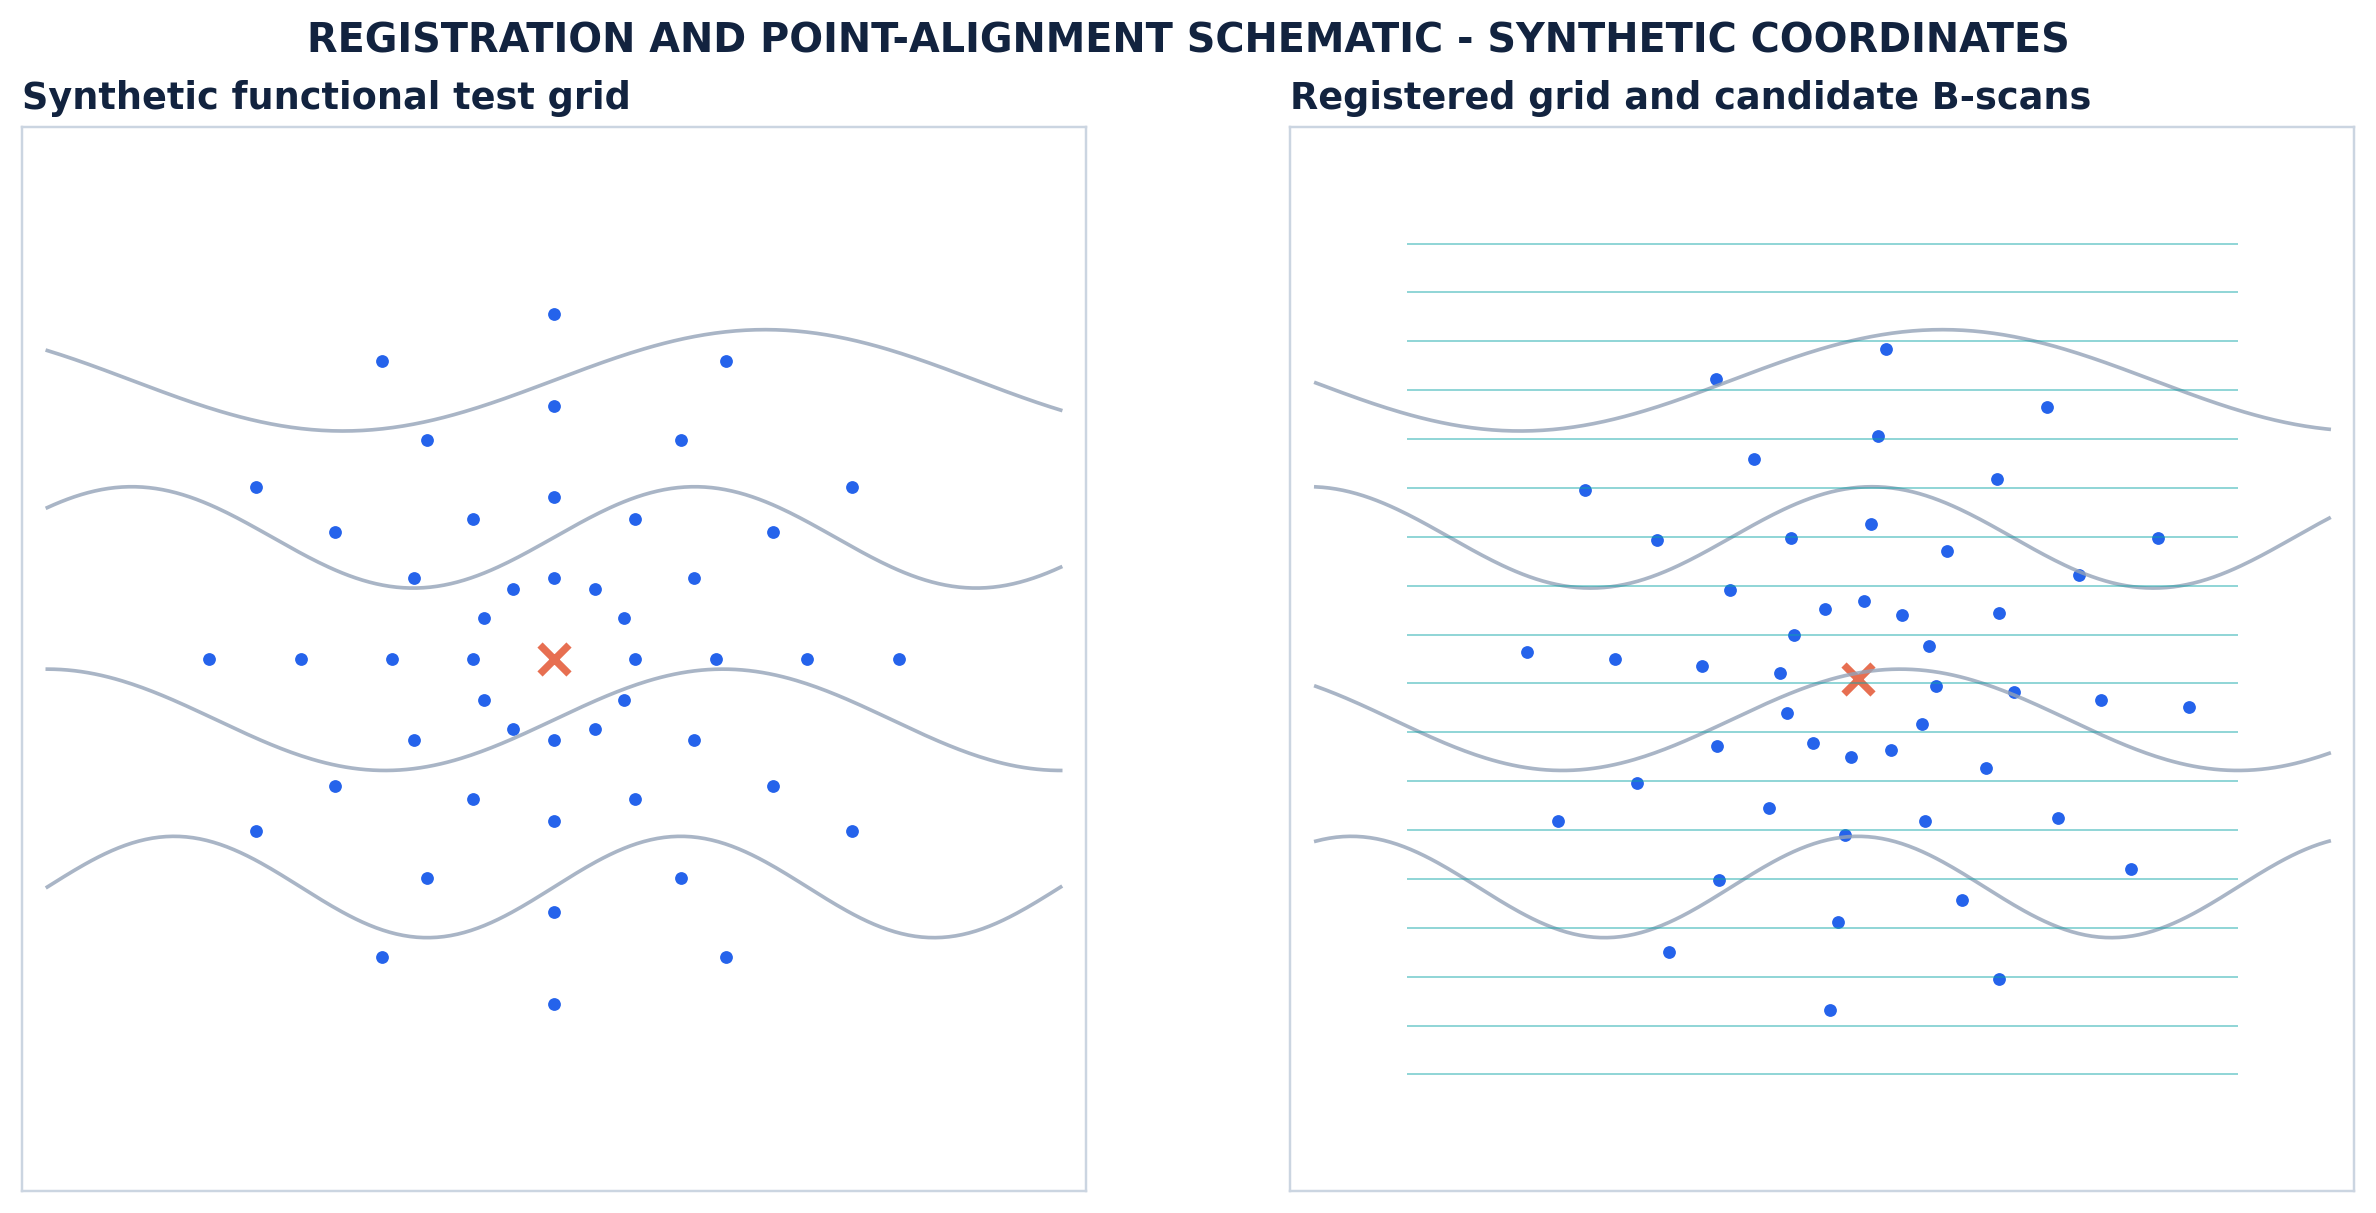
\includegraphics[width=\textwidth]{figure_registration_qc_public.png}
  \caption{Registration and point-alignment quality-control schematic using synthetic coordinates. The left panel represents a functional test grid; the right panel illustrates the registered grid and candidate B-scan geometry.}
  \label{fig:registration-qc}
\end{figure}

% -----------------------------------------------------------------------
\section{Point alignment and physical sampling}
\label{sec:footprint}

\subsection{Point-to-B-scan mapping}

The approved MAIA-to-OCT/SLO transform was applied to each numbered MAIA Point~1--37. For every transformed point, the three geometrically nearest OCT B-scan line segments were identified, and the projected along-scan coordinate, distance to the scan, B-scan identity and scan geometry were recorded. The choice of B-scans was based on geometry alone, without using OCT-derived features or sensitivity values.

Three B-scans were used so that the structure around a functional point could be represented from several immediately neighbouring cross-sections, limiting the influence of a small registration error, scan-placement variation or local imaging artefact in any one scan, while keeping the structural information local to the same MAIA location. Using substantially more scans would have made the representation less specific to the pointwise sensitivity measurement. The three selected scans were therefore treated as repeated structural views of one sensitivity label and combined before modelling, rather than as three independent labelled observations.

\subsection{Footprint anchor and local input definition}

The approximately 100~$\mu$m diameter of the MAIA stimulus was used to define the physical footprint around each registered point. For each selected B-scan, the registered MAIA point provided an along-scan coordinate. Scale X was used to express the $\pm50~\mu$m footprint in native image columns, and one centred native A-scan position within this interval was retained. This gave one local image anchor on each of the three B-scans and aligned the structural representation with the physical area represented by the functional measurement.

The retained A-scan position then centred a branch-specific OCT context image. The primary representation used a 750~$\mu$m horizontal context crop. The secondary boundary-aligned representation used a 300~$\mu$m horizontal context crop, with its vertical extent defined relative to the B0--B4 complex as described in Section~\ref{sec:representations}. The volume-specific horizontal scale preserved the intended physical extent across OCT volumes with different resolutions. Each crop was then resized to the input dimensions required by the feature extractor.

\subsection{Point-level representation and unit of modelling}

The analysis preserved the following hierarchy:

\begin{table}[htbp]
\centering
\caption{Hierarchical structure of one modelling observation.}
\label{tab:hierarchy}
\begin{tabularx}{\textwidth}{p{0.22\textwidth}X}
\toprule
Level & Meaning \\
\midrule
MAIA point & One sensitivity label in dB (the outcome) \\
B-scan & One of the three nearest registered scans \\
Local OCT context & One branch-specific context image centred on the selected native A-scan position \\
Model row & One structural representation per MAIA point \\
\bottomrule
\end{tabularx}
\end{table}

One embedding was extracted from each of the three local OCT contexts. These three embeddings were combined to produce one point-level representation for the corresponding MAIA sensitivity value. The neighbouring B-scans were therefore used as repeated structural views of the same point, without increasing the number of functional outcomes or treating them as independent observations.

\begin{figure}[htbp]
  \centering
  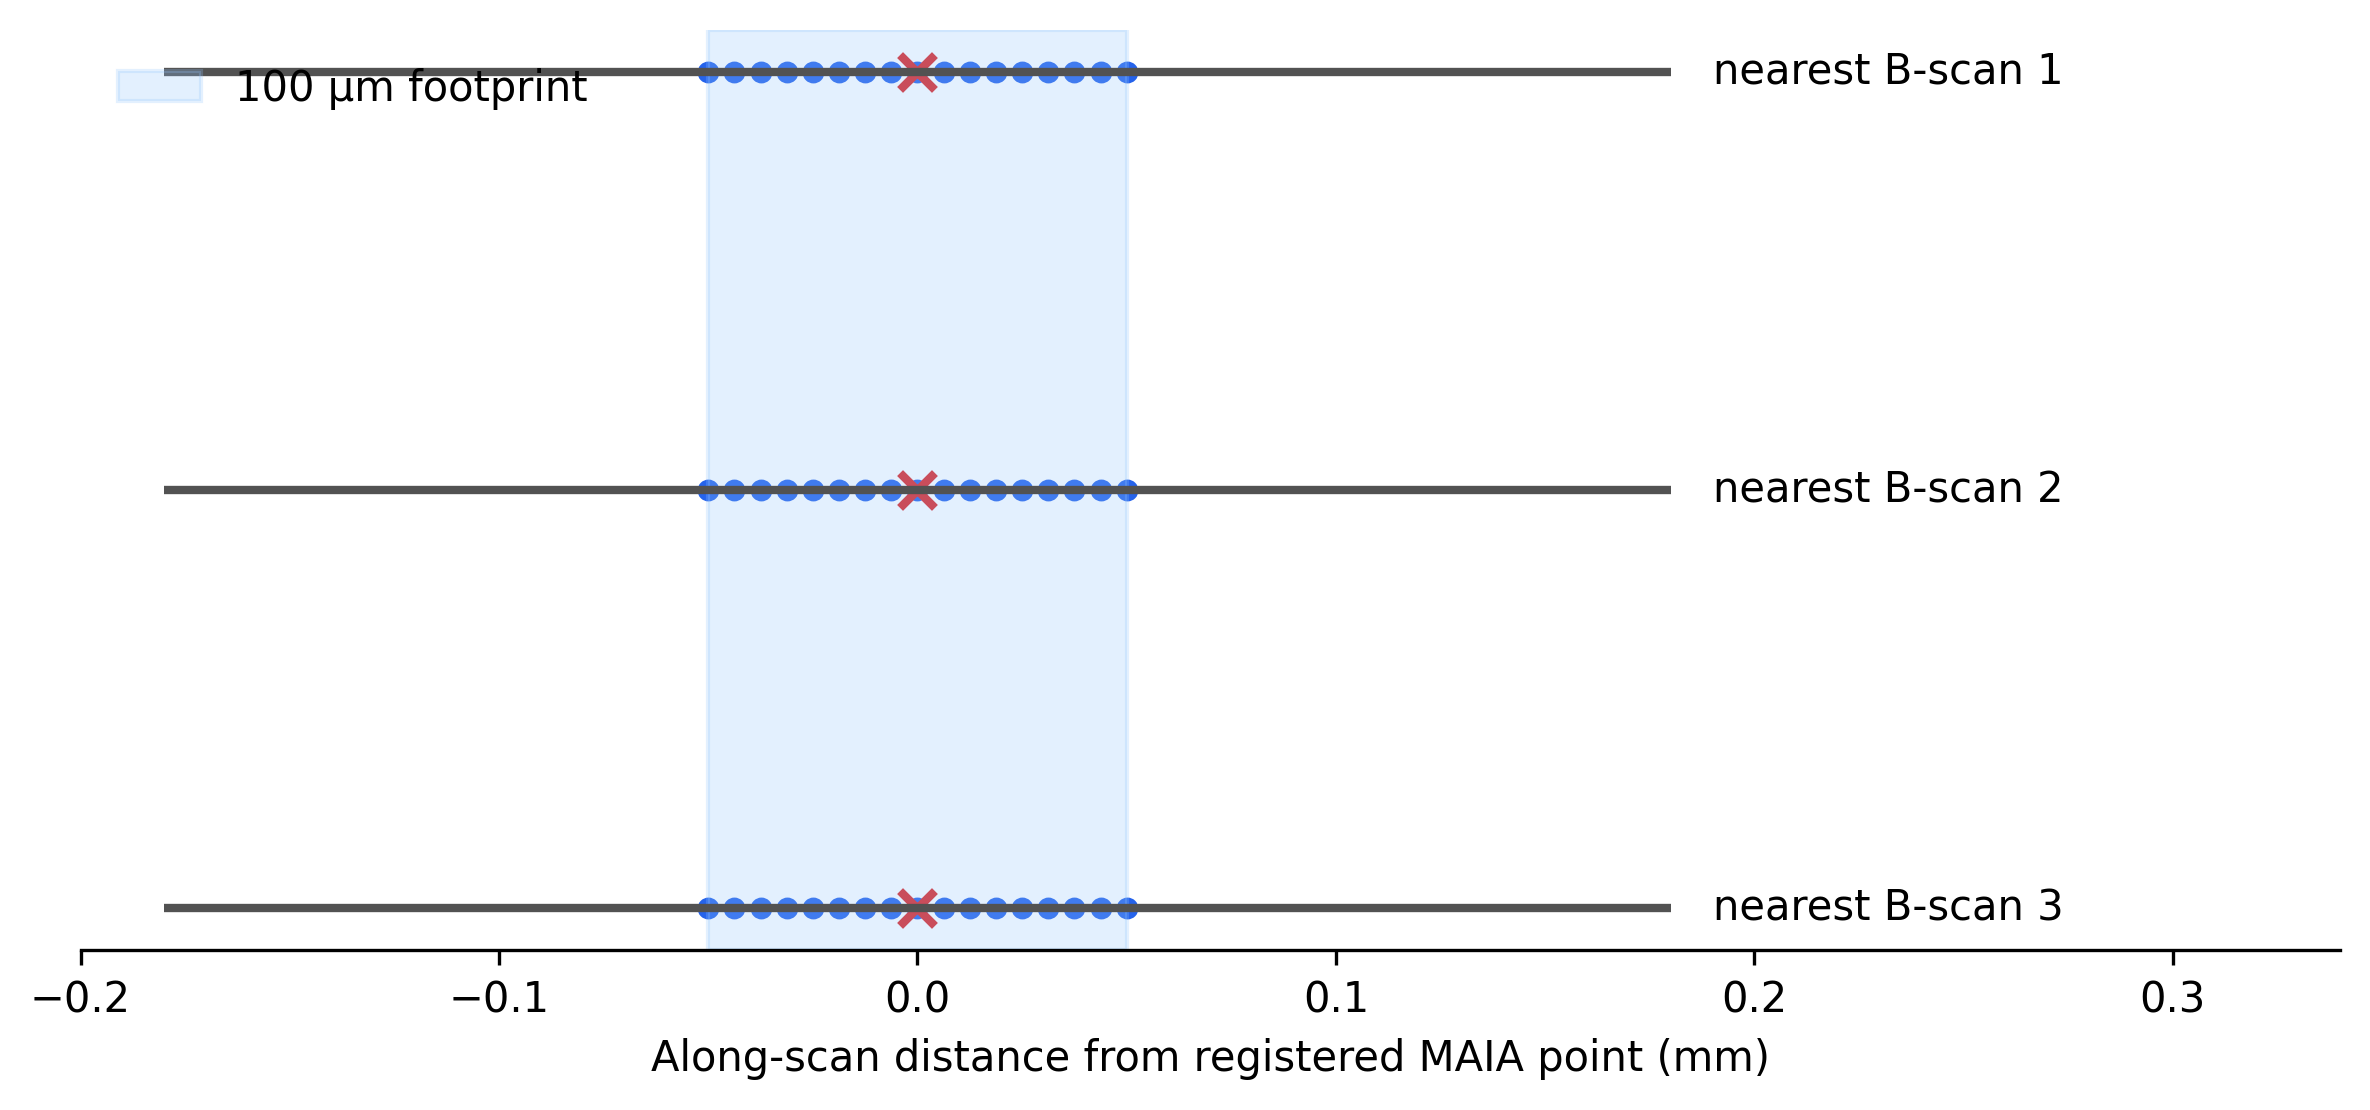
\includegraphics[width=0.92\linewidth]{figure_100um_sampling_primary.png}
  \caption{Footprint-aware pointwise OCT representation. One centred native A-scan position is selected within the approximately 100~$\mu$m MAIA footprint on each of the three nearest B-scans. A branch-specific encoder context is then centred on each selected position before the three structural views are combined.}
  \label{fig:footprint}
\end{figure}

% -----------------------------------------------------------------------
\section{OCT representations and feature construction}
\label{sec:representations}

Representation construction began once visit matching, registration, point projection, B-scan selection and footprint-based anchor selection had been completed. Because these spatial operations had already defined the local OCT input for each MAIA point, feature extraction could proceed on a consistent set of registered retinal contexts. The resulting representations were checked for identity, coverage and finite values before the corresponding sensitivity values were joined.

\subsection{Primary full-cohort image representation}

The primary branch included every accepted point and therefore used no boundary files or anatomical layer assignments. For each point, one centred native A-scan position was selected within the 100~$\mu$m footprint on each of the three selected B-scans. A 750~$\mu$m horizontal OCT context image was then centred on each position and passed to RETFound \citep{Zhou2023RETFound}, so that the representation captured structural information from the retinal region surrounding the functional measurement.

RETFound was used as a frozen feature extractor and evaluated in this Usher syndrome cohort alongside the prespecified reference models. The reasons for using a retinal foundation model are discussed in Chapter~\ref{chap:background}. As each point was represented on three B-scans, the resulting embeddings were summarised by their mean and population standard deviation, producing one $2{,}048$-dimensional point-level representation. This gave 8,658 encoder positions ($2{,}886$ points $\times$ 3 scans) and a final $2{,}886 \times 2{,}048$ representation for the primary cohort. Location was retained as a separate block using normalised eccentricity and the sine and cosine of polar angle, which represented the circular geometry of the test grid without an angular discontinuity.

\subsection{Secondary boundary-informed representation}

The secondary branch included observations with source-mapped B0--B4 curves that passed structural, mapping and gross-placement checks; these source labels were retained throughout the analysis.

Two complementary structural inputs were constructed for this branch:
\begin{itemize}[nosep]
  \item \textbf{Boundary features}, which summarised local distances and their variability within the measurement footprint; and
  \item \textbf{boundary-aligned RETFound features}, which represented the OCT image relative to the B0--B4 complex.
\end{itemize}

Four adjacent intervals were calculated from the B0--B4 curves within the 100~$\mu$m footprint. Their pooled means in $\mu$m, within-footprint standard deviations and between-B-scan mean standard deviations gave twelve boundary-derived features per point. These features described variation across the footprint and three selected scans, whereas the boundary-aligned RETFound representation used one centred A-scan anchor on each B-scan.

For the boundary-aligned image representation, OCT contexts were cropped relative to the B0--B4 complex, with fixed 50~$\mu$m margins above and below the complex and a 300~$\mu$m horizontal context. Each crop retained its physical aspect ratio before passing through the frozen RETFound encoder, and the three B-scan embeddings were then combined using the same point-level pooling rule.

\begin{table}[htbp]
\centering
\caption{Predictor representations used in each analysis branch.}
\label{tab:representations}
\begin{tabularx}{\textwidth}{p{0.27\textwidth}p{0.20\textwidth}p{0.22\textwidth}X}
\toprule
Representation & Cohort & Input & Purpose \\
\midrule
Location & Primary and secondary & Eccentricity and polar position & Transparent spatial reference \\
RETFound (standard) & Primary & Three local OCT contexts (one position on each selected B-scan) & Image-derived structural information \\
B0--B4 boundary features & Secondary only & Four adjacent neutral intervals and variability (12 features) & Interpretable structural branch \\
Boundary-aligned RETFound & Secondary only & OCT context aligned to B0--B4 complex & Image information relative to local boundaries \\
Fusion & Secondary only & Location, B0--B4 features and RETFound & Assessment of complementary information \\
\bottomrule
\end{tabularx}
\end{table}

% -----------------------------------------------------------------------
\section{Model development and comparators}
\label{sec:models}

The model set progressed from simple references to increasingly rich structural inputs:

\begin{itemize}[nosep]
  \item \textbf{Reference and location models} provided non-OCT benchmarks.
  \item \textbf{OCT and fusion models} tested structural information separately and in combination.
\end{itemize}

\subsection{Ridge regression and the choice of model family}

Ridge regression was used as the main fitted model because the independent sample consisted of 22 participants, even though the dataset contained 2,886 correlated point rows. A more flexible model could therefore learn patterns that were specific to the participants in this cohort, whereas ridge regression provides shrinkage for correlated predictors while remaining relatively easy to interpret. Within each outer training set, the 2,048-dimensional RETFound vector was standardised with the training-fold scaler and reduced using principal component analysis (PCA). PCA was fitted on training data only, with whitening and a fixed random state, and the number of retained components was selected from $\{8, 16, 32, 64, 128\}$ using grouped inner-fold mean absolute error. The ridge penalty was selected from $\alpha \in \{0.1, 1, 10, 100, 1000\}$ using the same criterion. Location features were standardised in the same way but were not reduced with PCA because this block contained only three prespecified variables. Predictions were retained on the scale produced by the fitted model.

\subsection{Primary model ladder}

Five models were specified for the primary analysis. The training-mean null model showed the error obtained when every held-out point was assigned the mean sensitivity of the training participants, while the fixed $-1$~dB reference provided a simple non-learned comparison at the measurement floor. The location-only ridge model then measured the information available from retinal position without OCT. RETFound-only and location-plus-RETFound ridge models assessed the image-derived representation without and with explicit location information; together, these comparisons indicated whether image-derived information improved prediction beyond retinal position.

\begin{table}[htbp]
\centering
\caption{Primary model ladder and the inferential question addressed by each model.}
\label{tab:primary-ladder}
\begin{tabularx}{\textwidth}{p{0.33\textwidth}X}
\toprule
Model & Purpose \\
\midrule
Training-mean null & Reference error when prediction uses only the training-participant mean \\
Fixed $-1$~dB reference & Non-learned sensitivity-floor reference \\
Location-only ridge & Information from point location without OCT \\
RETFound-only ridge & Frozen image representation without explicit location predictors \\
Location-plus-RETFound ridge & Primary combined model; added value of OCT beyond location \\
\bottomrule
\end{tabularx}
\end{table}

\subsection{Secondary model ladder}

The secondary analysis used the same separation of training and test participants, but was carried out on the subset with boundary information. It therefore expanded the model set to nine models. Ordinary linear regression provided a simple, interpretable boundary baseline, while ridge regression considered the same features with shrinkage for correlated intervals and variability measures. Random forest was included as a non-linear comparison because the relation between local structural measurements and sensitivity might not be additive; it used 500 trees during inner tuning and 1,000 trees for the final selected fit. Boundary-aligned RETFound then tested image-derived information alongside the engineered structural summary, and the fusion model assessed whether location, boundary features and image information were complementary.

\begin{table}[htbp]
\centering
\caption{Secondary model ladder and the inferential question addressed by each model.}
\label{tab:secondary-ladder}
\begin{tabularx}{\textwidth}{p{0.38\textwidth}X}
\toprule
Model & Purpose \\
\midrule
Training-mean null; fixed $-1$~dB reference & Learned and non-learned baselines under the same held-out participants \\
Location-only ridge & Contribution of retinal position alone \\
Boundary-only linear regression & Simplest interpretable linear test of the 12 neutral boundary predictors \\
Boundary-only ridge & Same structural block with shrinkage for correlated features \\
Location-plus-boundary ridge & Early fusion; incremental structural value beyond location \\
Location-plus-boundary random forest & Flexible non-linear test for interactions missed by ridge \\
Boundary-aligned RETFound ridge & Image features at boundary-aligned positions without location or boundary predictors \\
Location-plus-boundary RETFound ridge & Early fusion of location, boundary features and image representation \\
\bottomrule
\end{tabularx}
\end{table}

% -----------------------------------------------------------------------
\section{Validation, evaluation and uncertainty}
\label{sec:validation}

\subsection{Participant-grouped nested validation}

Five outer folds were fixed using participant identifier as the allocation unit. The deterministic allocation aimed to balance the numbers of accepted eye-visits and visit timepoints, without using sensitivity values, OCT images, OCT features or registration-quality scores. All eyes, visits, MAIA points, B-scan assignments and representations belonging to one participant were placed in the same outer fold.

For each outer fold, the held-out participants were used only for the final prediction. The remaining participants supplied the training data for model fitting and configuration decisions. Splitting at point level could place correlated observations, fellow-eye data or repeat visits from one participant in both training and testing. This would make the estimate of performance appear better than it would be for a new participant.

Within each outer training set, four grouped inner folds were used to select model hyperparameters. The final model for that outer split was then fitted using all outer-training participants and the selected configuration. It was used once to predict the held-out participants. Repeating this procedure across the five outer folds gave one out-of-fold prediction for every point and model. Imputation, scaling, PCA transformation, ridge fitting and hyperparameter selection were all restricted to the relevant training data. The completed primary run contained 14,430 prediction rows: 2,886 points for each of the five models.

\subsection{Evaluation metrics}

All performance measures were calculated from the out-of-fold predictions. Let $\hat{y}_i$ denote the predicted sensitivity and $y_i$ the observed sensitivity for point $i$. Mean absolute error (MAE) is

\begin{equation}
  \mathrm{MAE} = \frac{1}{n}\sum_{i=1}^{n}\left|\hat{y}_i - y_i\right|,
\end{equation}

and root mean squared error (RMSE) is

\begin{equation}
  \mathrm{RMSE} = \sqrt{\frac{1}{n}\sum_{i=1}^{n}\left(\hat{y}_i - y_i\right)^2}.
\end{equation}

MAE was used as the primary ranking metric because it is expressed directly in dB and is less affected by a small number of large errors than RMSE. RMSE was reported alongside it to show the effect of larger deviations.

For the Bland--Altman analysis, the difference was defined as predicted minus observed sensitivity, $d_i = \hat{y}_i - y_i$. A positive bias therefore means that the predictions are higher than the observations. Bias is the mean difference, and the 95\% limits of agreement are calculated as the bias $\pm 1.96$ times the standard deviation of the differences. Calibration intercept and slope were obtained by regressing observed sensitivity on predicted sensitivity. $R^2$ was also calculated as a supplementary descriptive measure. The role and limitation of each metric are summarised in Table~\ref{tab:metrics}.

\begin{table}[htbp]
\centering
\caption{Evaluation metrics, their primary roles and what each cannot support on its own.}
\label{tab:metrics}
\begin{tabularx}{\textwidth}{p{0.27\textwidth}p{0.30\textwidth}X}
\toprule
Metric & Role & Limitation \\
\midrule
MAE (dB) & Primary ranking; absolute pointwise error & Does not reveal direction of error \\
RMSE (dB) & Sensitivity to larger errors & Dominated by outliers; not in dB of clinical intuition \\
Bland--Altman bias (dB) & Average directional error & Does not capture individual-point scatter \\
95\% limits of agreement (dB) & Individual-point agreement range & Cannot establish clinical interchangeability alone \\
Calibration intercept / slope & Systematic over- or under-prediction & Requires error and agreement to interpret \\
$R^2$ & Supplementary explained variance & A favourable value can coexist with wide pointwise limits \\
\bottomrule
\end{tabularx}
\end{table}

\subsection{Uncertainty and prespecified descriptive strata}

Uncertainty intervals were obtained with 5,000 participant-level bootstrap resamples. In each draw, participants were sampled with replacement and all of their associated points and visits were included with the corresponding multiplicity. This preserved the clustered structure of the data, which would be lost in a point-level bootstrap. The 2.5th and 97.5th percentiles of the bootstrap distribution formed the reported 95\% interval.

Four descriptive strata were specified in advance: baseline visit, year-one visit, observations at the $-1$~dB device floor and observations above the floor. These strata show where prediction errors occurred and how the floor affected interpretation. They are not additional primary endpoints, and differences between strata are not treated as confirmatory subgroup effects.

% -----------------------------------------------------------------------
\section{Data governance and ethical considerations}
\label{sec:ethics}

This study used pre-existing, de-identified OCT and MAIA microperimetry data. The records were organised using study-specific identifiers, and direct identifiers were not included in the analytical dataset or thesis materials. No new data were collected for this project, and the analysis did not inform clinical decisions.

The model outputs are research estimates of pointwise retinal sensitivity. They are intended to support the evaluation of OCT--function relationships in this cohort and require further validation before any clinical use could be considered.

\chapter{Results}
\label{chap:results}

\section{Primary full-cohort model comparison}
\label{sec:primary-results}

All five primary models generated one participant-held-out prediction for each of the 2,886 points. The location-plus-RETFound ridge had the lowest MAE at 5.485~dB (95\% CI 4.871--6.177), followed by RETFound-only ridge at 5.652~dB (95\% CI 5.080--6.273). As the location-only ridge achieved an MAE of 7.650~dB (95\% CI 6.829--8.440), adding the image representation was associated with a 2.165~dB reduction in MAE. The combined model had an RMSE of 6.986~dB, a calibration slope of 0.978 and a supplementary $R^2$ of 0.564. Its mean prediction-minus-observation bias was $-0.060$~dB, while the limits of agreement ranged from $-13.754$ to 13.634~dB.

\begin{table}[htbp]
\centering
\footnotesize
\caption{Primary all-cohort out-of-fold performance (22 participants, 78 eye-visits and 2,886 points). MAE confidence intervals are participant-bootstrap 95\% intervals. Bias is prediction minus observed sensitivity; $R^2$ is supplementary.}
\label{tab:primary-performance}
\renewcommand{\arraystretch}{1.18}
\setlength{\tabcolsep}{3pt}
\begin{tabular}{@{}>{\raggedright\arraybackslash}p{0.22\textwidth}>{\centering\arraybackslash}p{0.18\textwidth}>{\centering\arraybackslash}p{0.11\textwidth}>{\centering\arraybackslash}p{0.13\textwidth}>{\centering\arraybackslash}p{0.19\textwidth}>{\centering\arraybackslash}p{0.08\textwidth}@{}}
\toprule
Model & \shortstack{MAE, dB\\(95\% CI)} & \shortstack{RMSE,\\dB} & \shortstack{Bias,\\dB} & \shortstack{95\% limits of\\agreement, dB} & $R^2$ \\
\midrule
Training-mean null & 9.346 (8.633--10.104) & 10.596 & 0.004 & $-20.769$ to 20.776 & $-0.004$ \\
Fixed $-1$~dB reference & 17.076 (13.969--20.166) & 20.086 & $-17.076$ & $-37.809$ to 3.658 & $-2.606$ \\
Location-only ridge & 7.650 (6.829--8.440) & 9.048 & 0.004 & $-17.732$ to 17.740 & 0.268 \\
RETFound-only ridge & 5.652 (5.080--6.273) & 7.146 & $-0.245$ & $-14.246$ to 13.755 & 0.543 \\
Location-plus-RETFound ridge & 5.485 (4.871--6.177) & 6.986 & $-0.060$ & $-13.754$ to 13.634 & 0.564 \\
\bottomrule
\end{tabular}
\end{table}

Figure~\ref{fig:primary-model-comparison} presents the same comparison with the participant-bootstrap intervals. The two image-based ridge models are clearly separated from the location-only and training-mean references, whereas their intervals overlap each other. The location-plus-RETFound ridge therefore has the lowest observed MAE in the primary ladder, but its numerical advantage over RETFound-only ridge is small relative to the uncertainty shown in the figure. The fixed $-1$~dB reference has the highest error and the widest interval, as it assigns the same value to every point regardless of its observed sensitivity or location.

\begin{figure}[htbp]
  \centering
  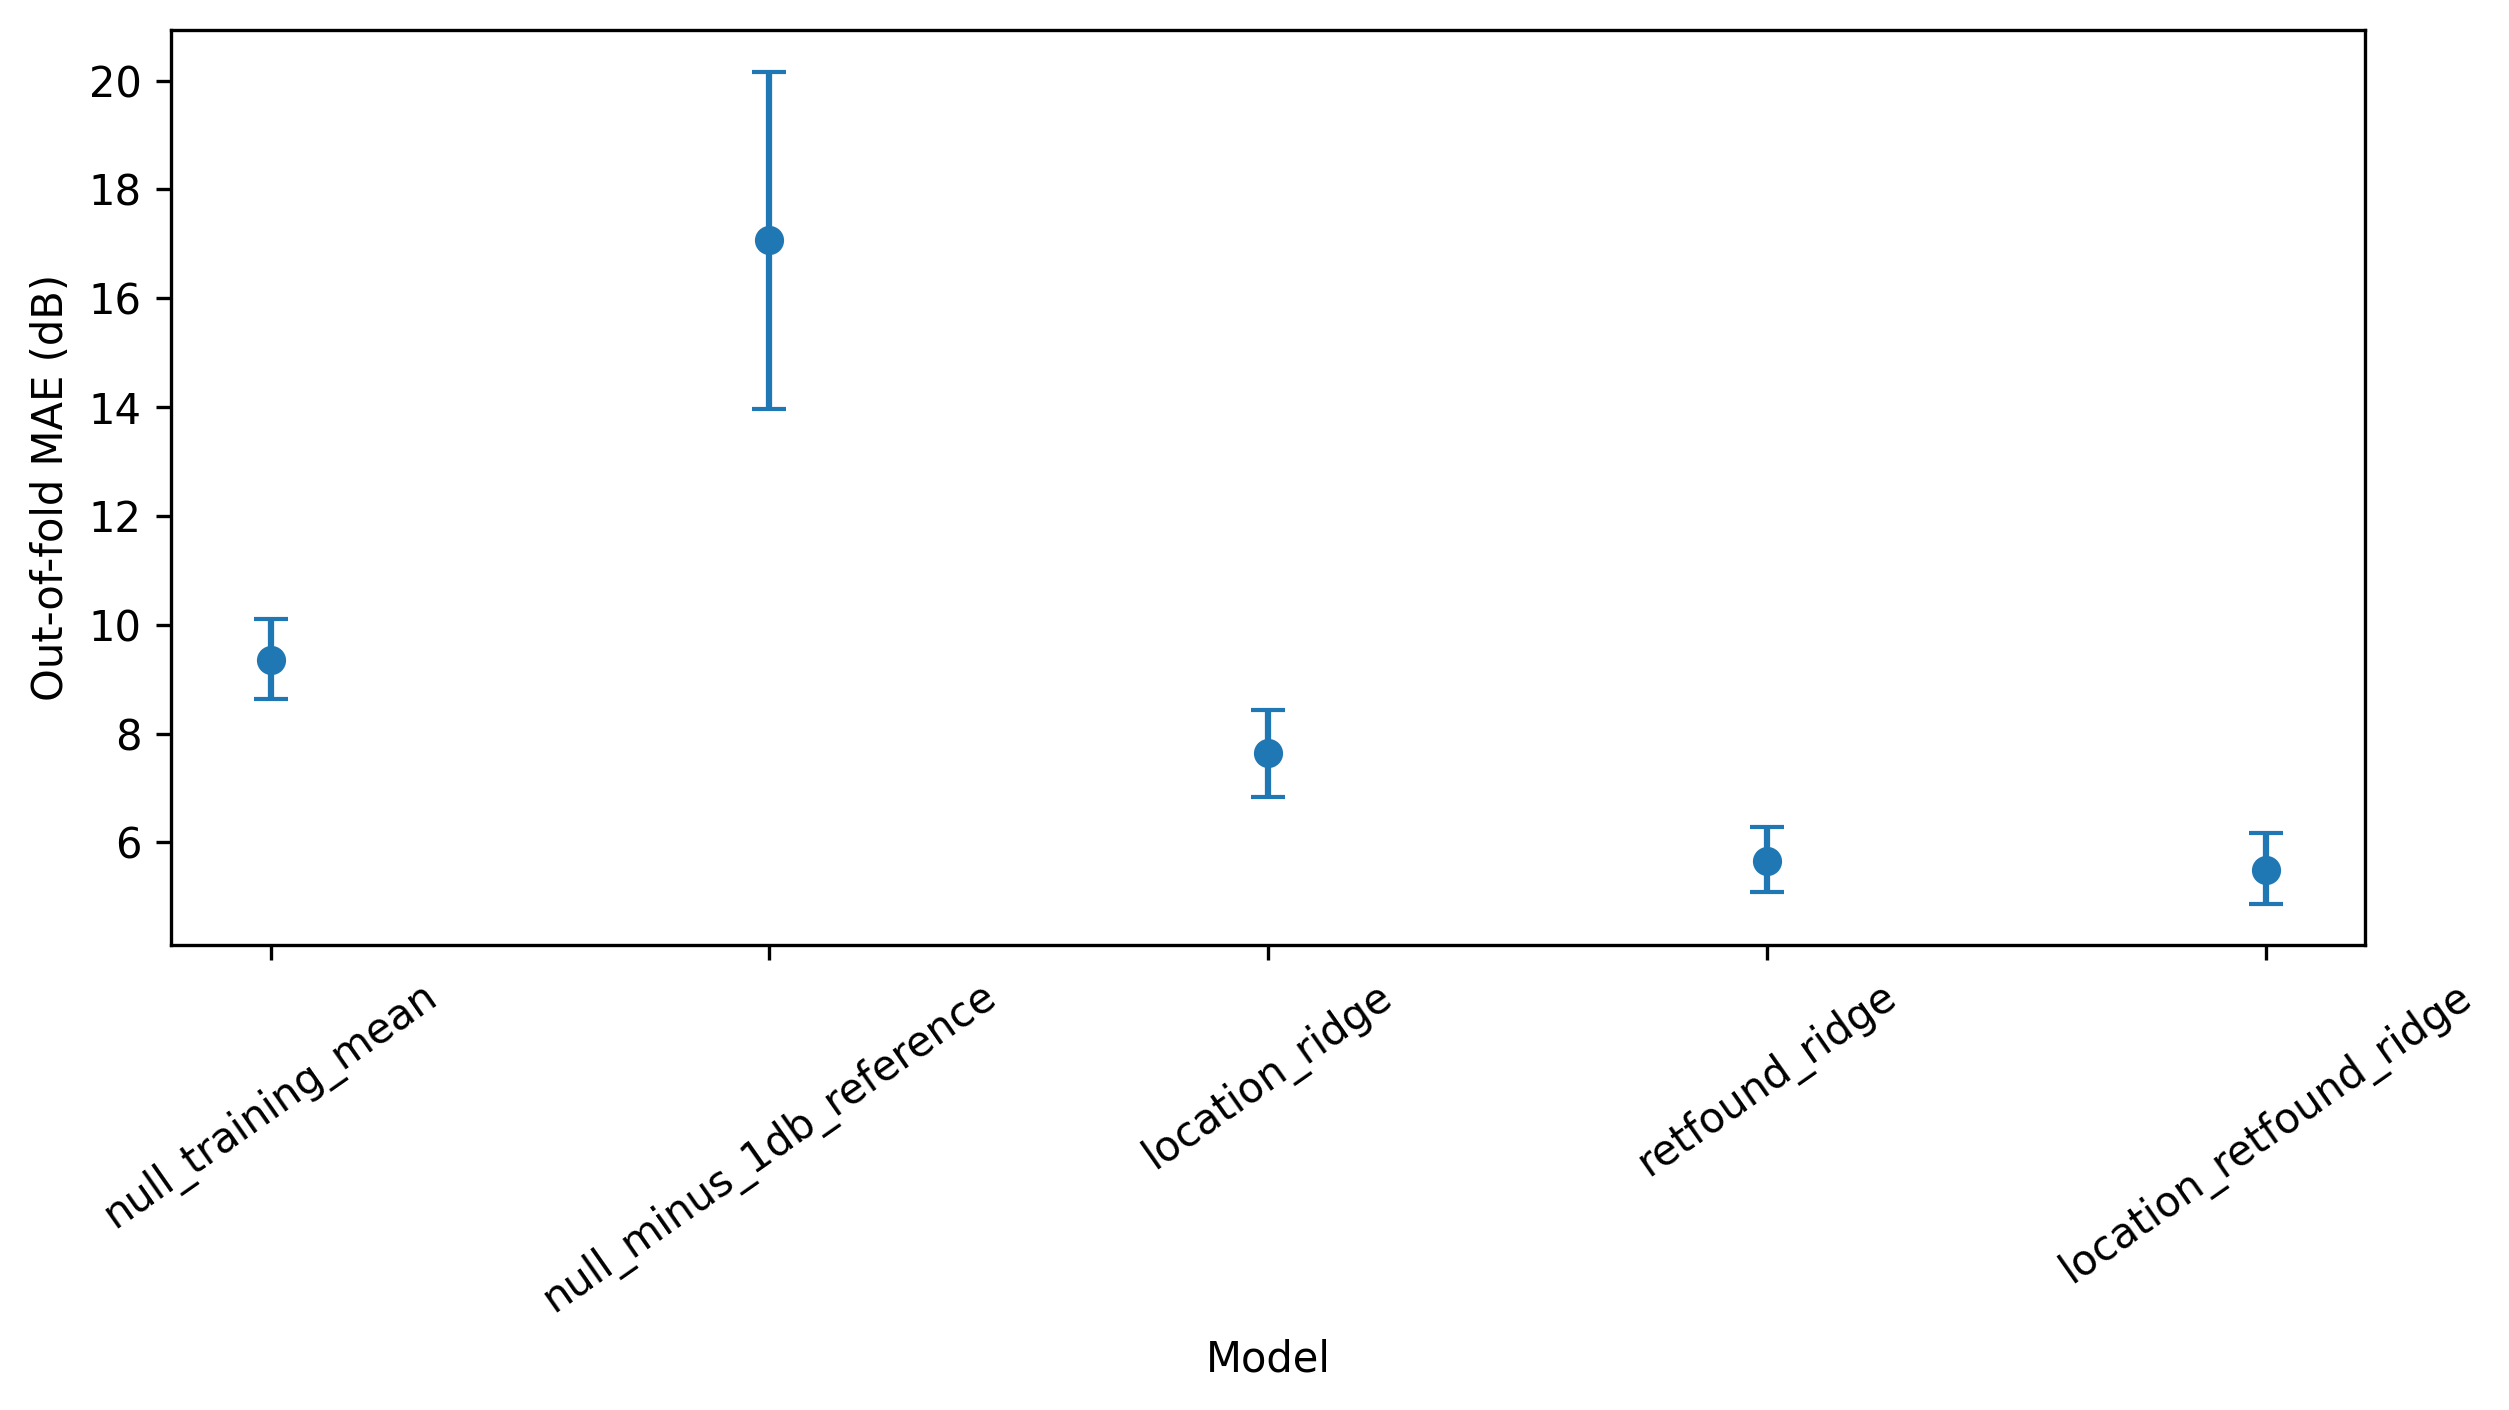
\includegraphics[width=0.95\linewidth]{figure_primary_model_comparison.png}
  \caption{Participant-bootstrap MAE comparison for the five primary models. Lower values indicate lower pointwise error; the location-plus-RETFound ridge is the best primary model by MAE.}
  \label{fig:primary-model-comparison}
\end{figure}

\begin{figure}[htbp]
  \centering
  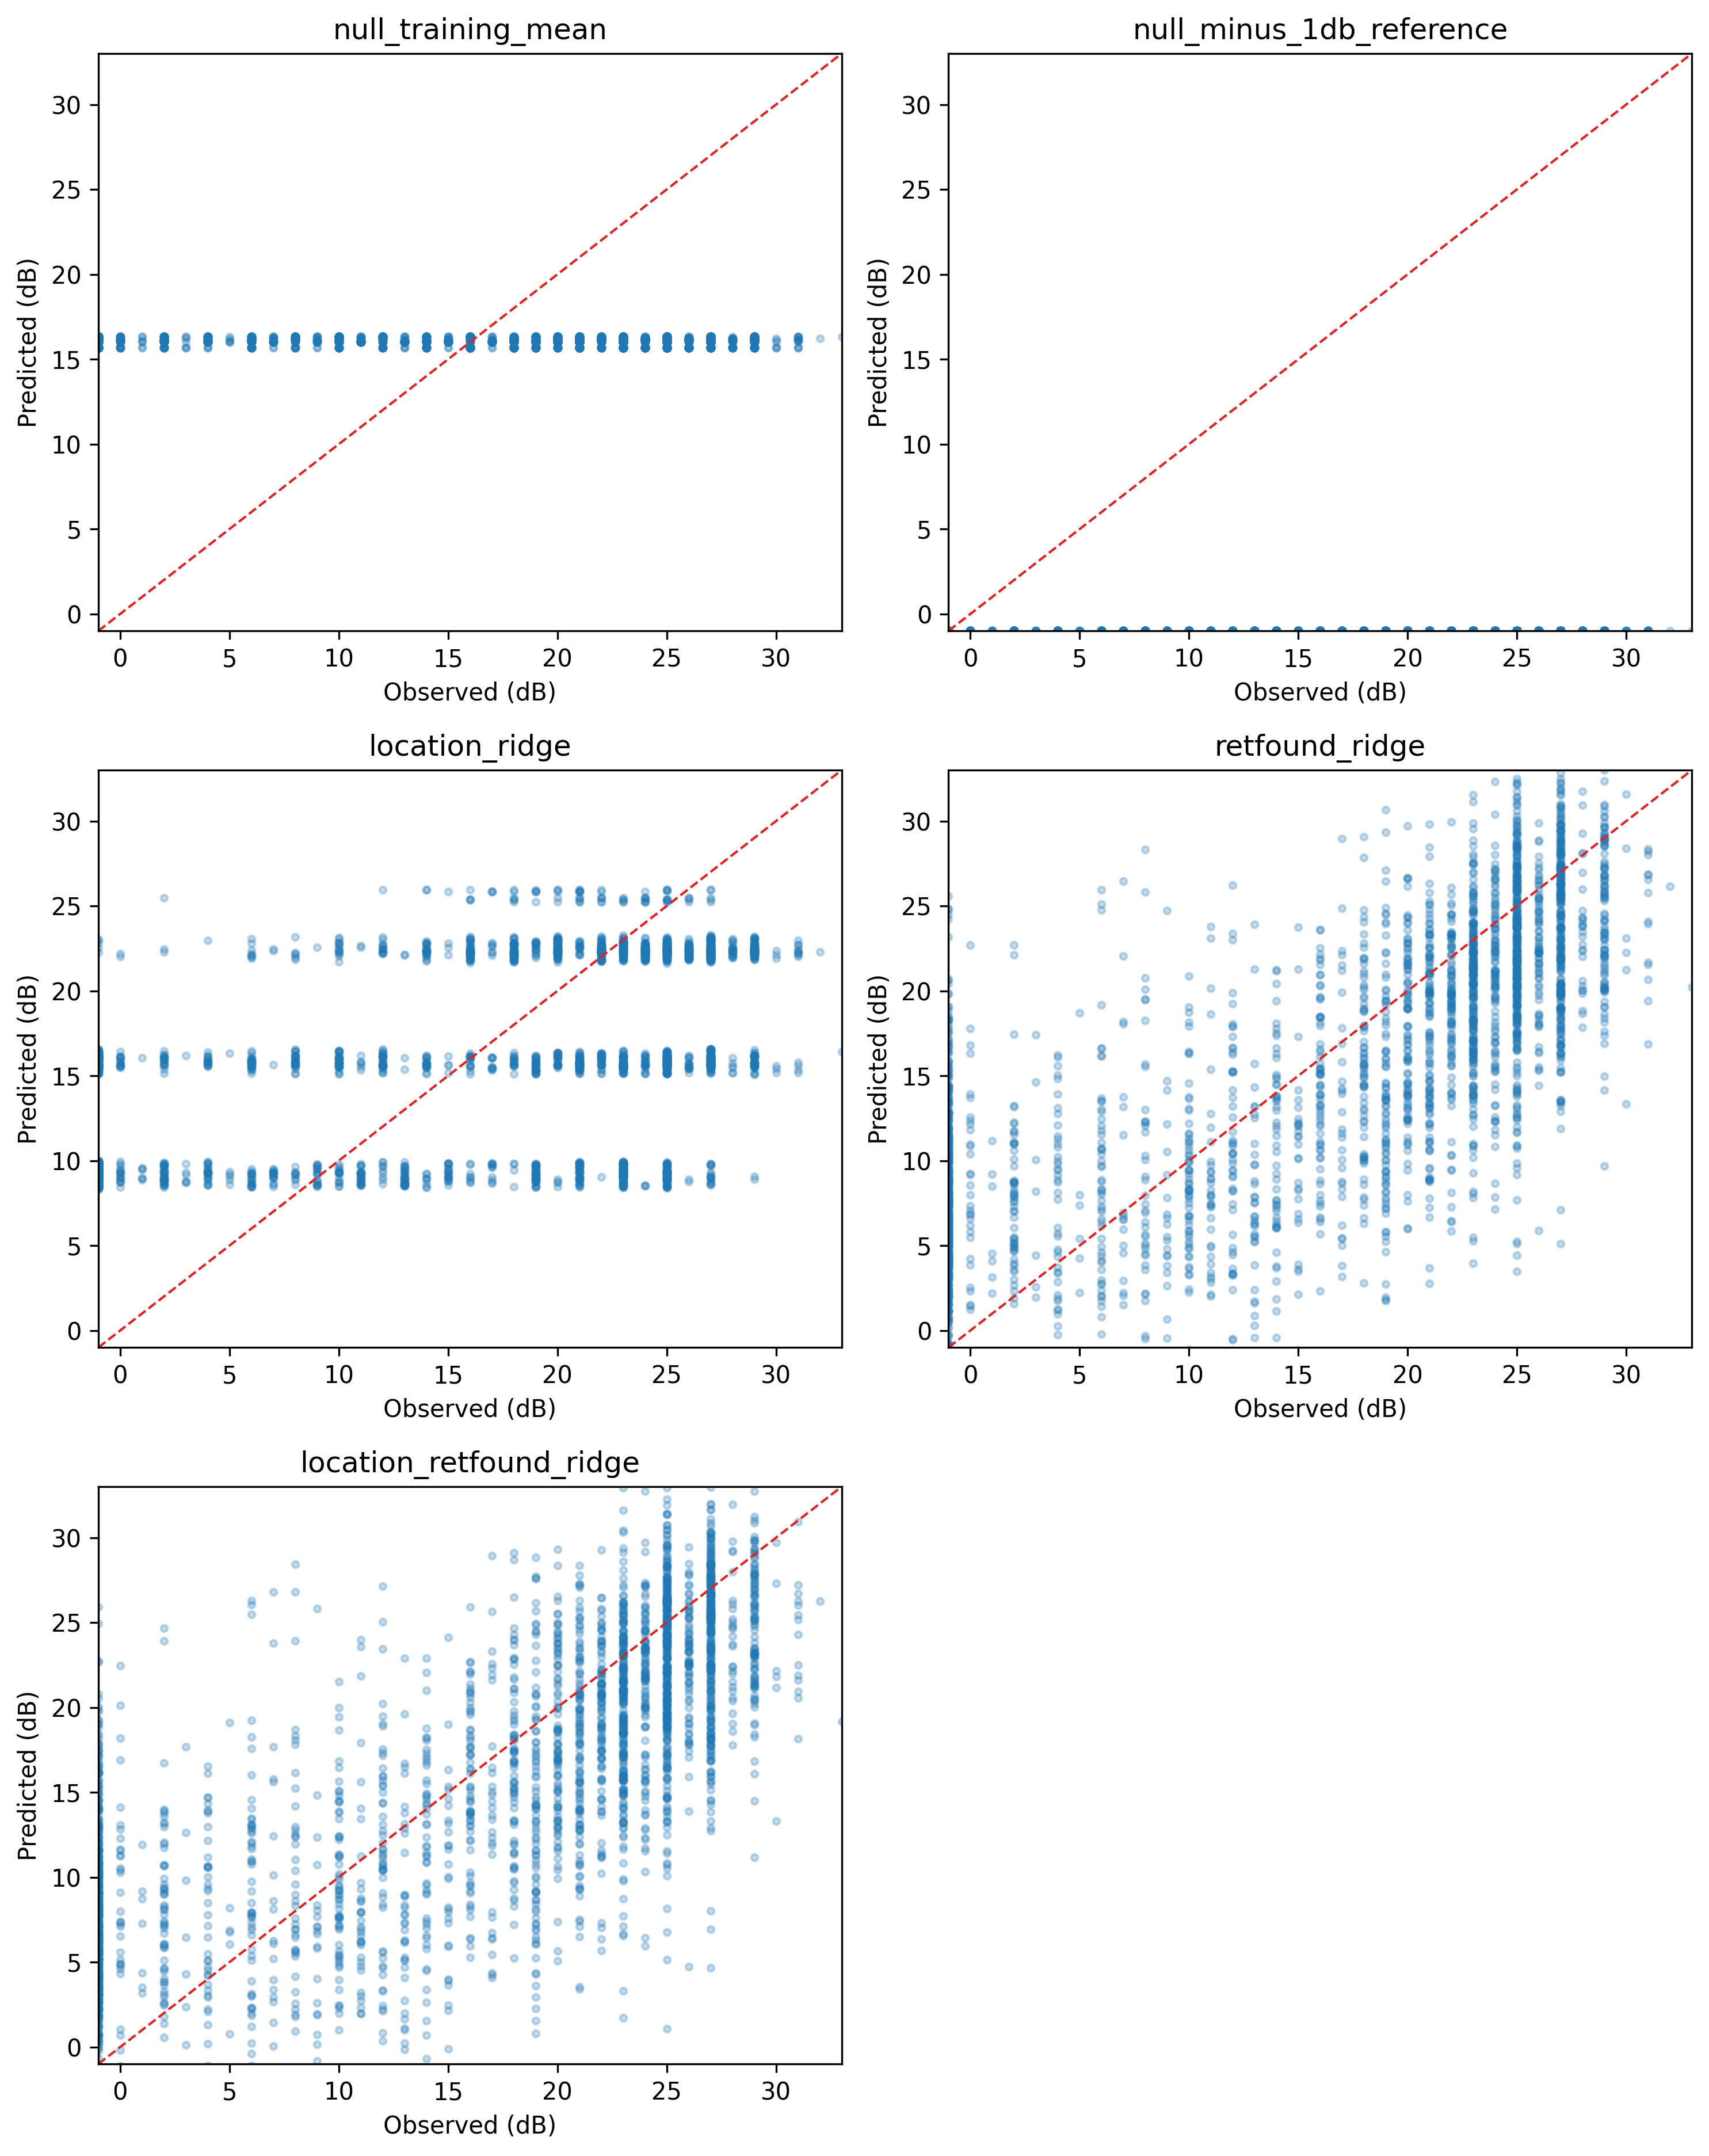
\includegraphics[width=0.98\linewidth,height=0.62\textheight,keepaspectratio]{figure_primary_observed_predicted.png}
  \caption{Observed versus out-of-fold predicted pointwise sensitivity for the primary model ladder. The repeated horizontal accumulation at $-1$~dB reflects the MAIA device floor.}
  \label{fig:primary-observed-predicted}
\end{figure}

The observed-versus-predicted panels in Figure~\ref{fig:primary-observed-predicted} show the change in prediction behaviour across the ladder. The training-mean and fixed-reference panels appear as horizontal bands because neither model varies its prediction with the observed point. The location-only model produces several broad horizontal groupings, reflecting the restricted set of predictions available from fixed grid location. In contrast, both RETFound models cover a much wider range of predicted sensitivities and show an upward pattern relative to the diagonal reference line. The location-plus-RETFound model places more of its predictions near this line at the higher observed sensitivities, although substantial vertical spread remains at individual sensitivity values. The dense vertical accumulation at $-1$~dB is visible in each fitted model and corresponds to the device-floor observations.

\begin{figure}[htbp]
  \centering
  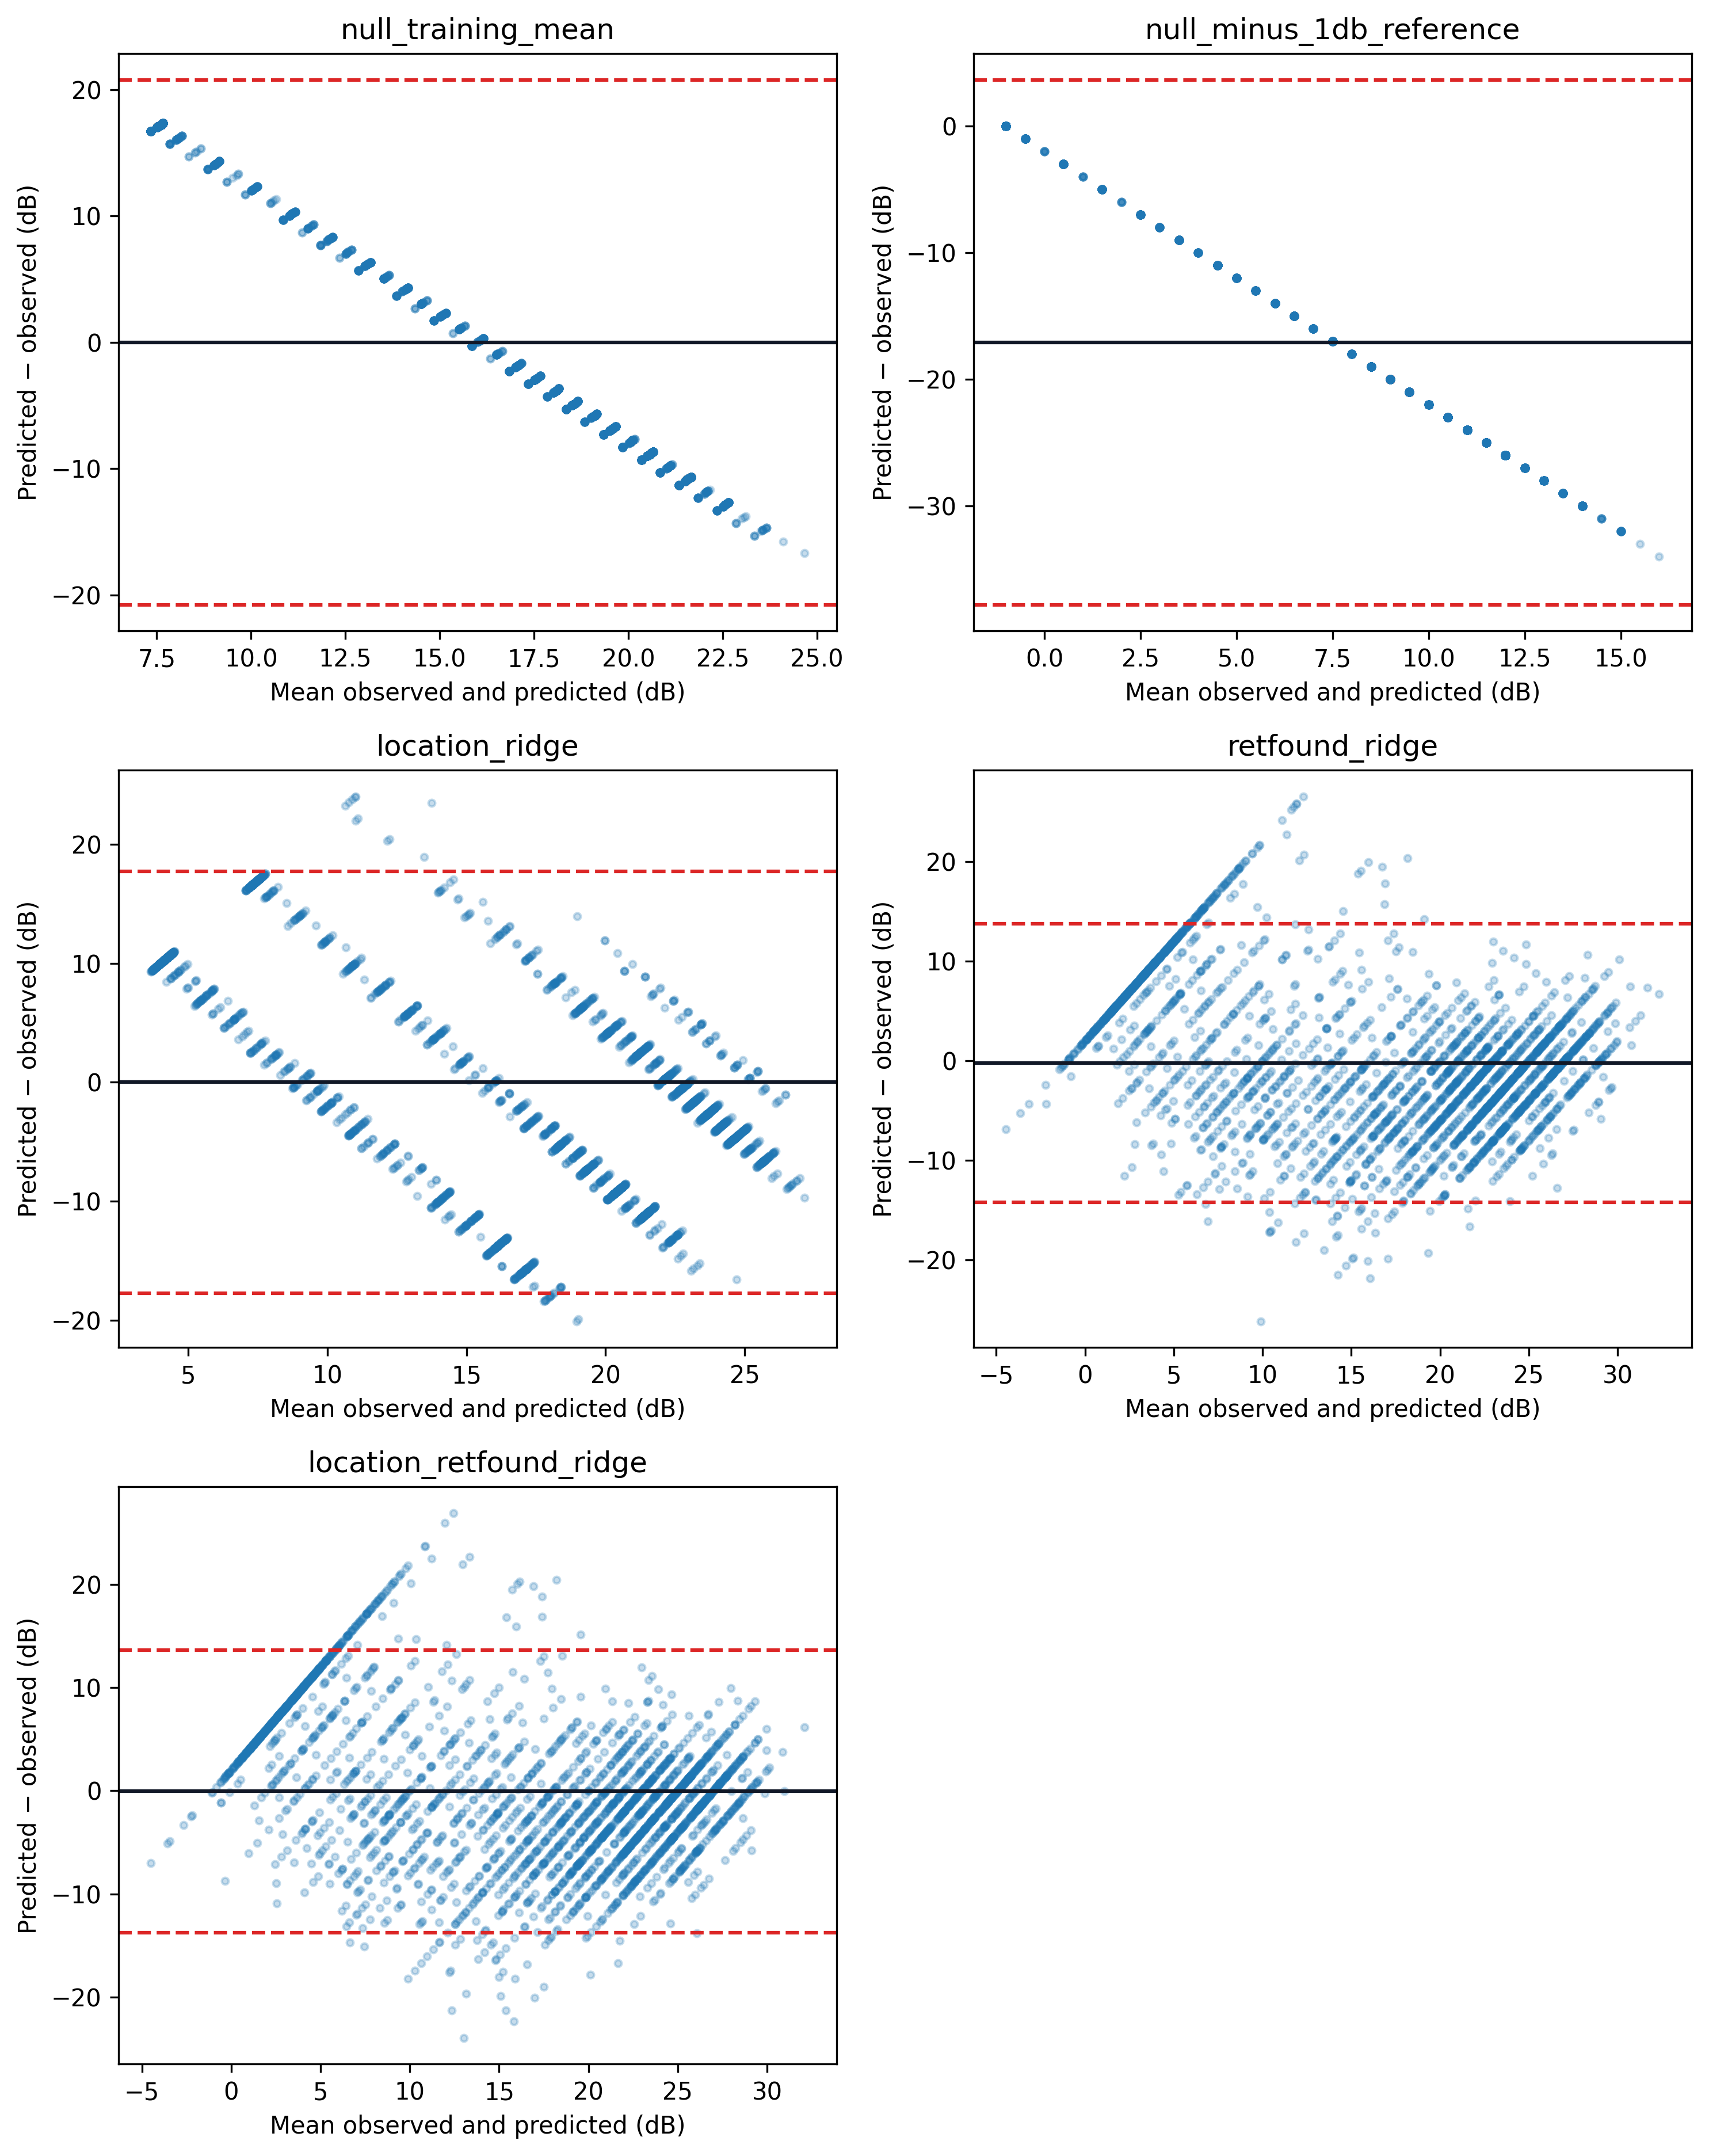
\includegraphics[width=0.98\linewidth,height=0.62\textheight,keepaspectratio]{figure_primary_bland_altman.png}
  \caption{Bland--Altman plots for the primary model ladder. Differences are prediction minus observed sensitivity.}
  \label{fig:primary-bland-altman}
\end{figure}

Figure~\ref{fig:primary-bland-altman} gives the same comparisons on the prediction-minus-observation scale. The two non-imaging references show the expected deterministic diagonal patterns, while the location-only model retains grouped residual bands. The image-based models have residuals distributed on both sides of zero across much of the range, and the location-plus-RETFound ridge is centred close to zero overall. The plot also shows that errors remain dispersed: at the lowest observed values, including the floor, many predictions are above the measured sensitivity, whereas negative residuals are more common at higher observed sensitivities. This visible pattern is consistent with the reported limits of agreement and complements the small overall bias.

\section{Primary error strata and calibration}

Descriptive error differed across the prespecified strata. The location-plus-RETFound ridge had a lower MAE at year one than at baseline (4.998 versus 5.925~dB), although the two visits contained different numbers of participants and points. Error was also higher for observations at the $-1$~dB device floor, where MAE was 8.787~dB, than for observations above the floor, where MAE was 4.737~dB. The floor stratum contained 533 points from 16 participants, whereas the non-floor stratum contained 2,353 points from all 22 participants.

\begin{table}[htbp]
\centering
\caption{Location-plus-RETFound ridge error by prespecified stratum. Values are descriptive out-of-fold summaries.}
\label{tab:primary-strata}
\begin{tabularx}{\textwidth}{Xrrrr}
\toprule
Stratum & Participants & Points & MAE, dB & RMSE, dB \\
\midrule
Baseline visit & 22 & 1,517 & 5.925 & 7.534 \\
Year-one visit & 20 & 1,369 & 4.998 & 6.323 \\
Sensitivity floor ($-1$~dB) & 16 & 533 & 8.787 & 9.948 \\
Above sensitivity floor & 22 & 2,353 & 4.737 & 6.119 \\
\bottomrule
\end{tabularx}
\end{table}

The residual plot in Figure~\ref{fig:primary-residuals} makes the floor-related pattern more apparent. For the location-plus-RETFound model, the column of observations at $-1$~dB includes a broad range of positive errors, while the range of residuals remains wider than zero across the middle and upper sensitivity values. This agrees with the stratum summaries in Table~\ref{tab:primary-strata}: the floor group had the largest MAE and RMSE. Figure~\ref{fig:primary-sensitivity-distribution} shows why this group is consequential in the full cohort. There is a pronounced spike at the device floor, alongside a broad concentration of values in the higher-sensitivity range, particularly around 20--27~dB. The endpoint is therefore not evenly distributed across its observed range.

\begin{figure}[htbp]
  \centering
  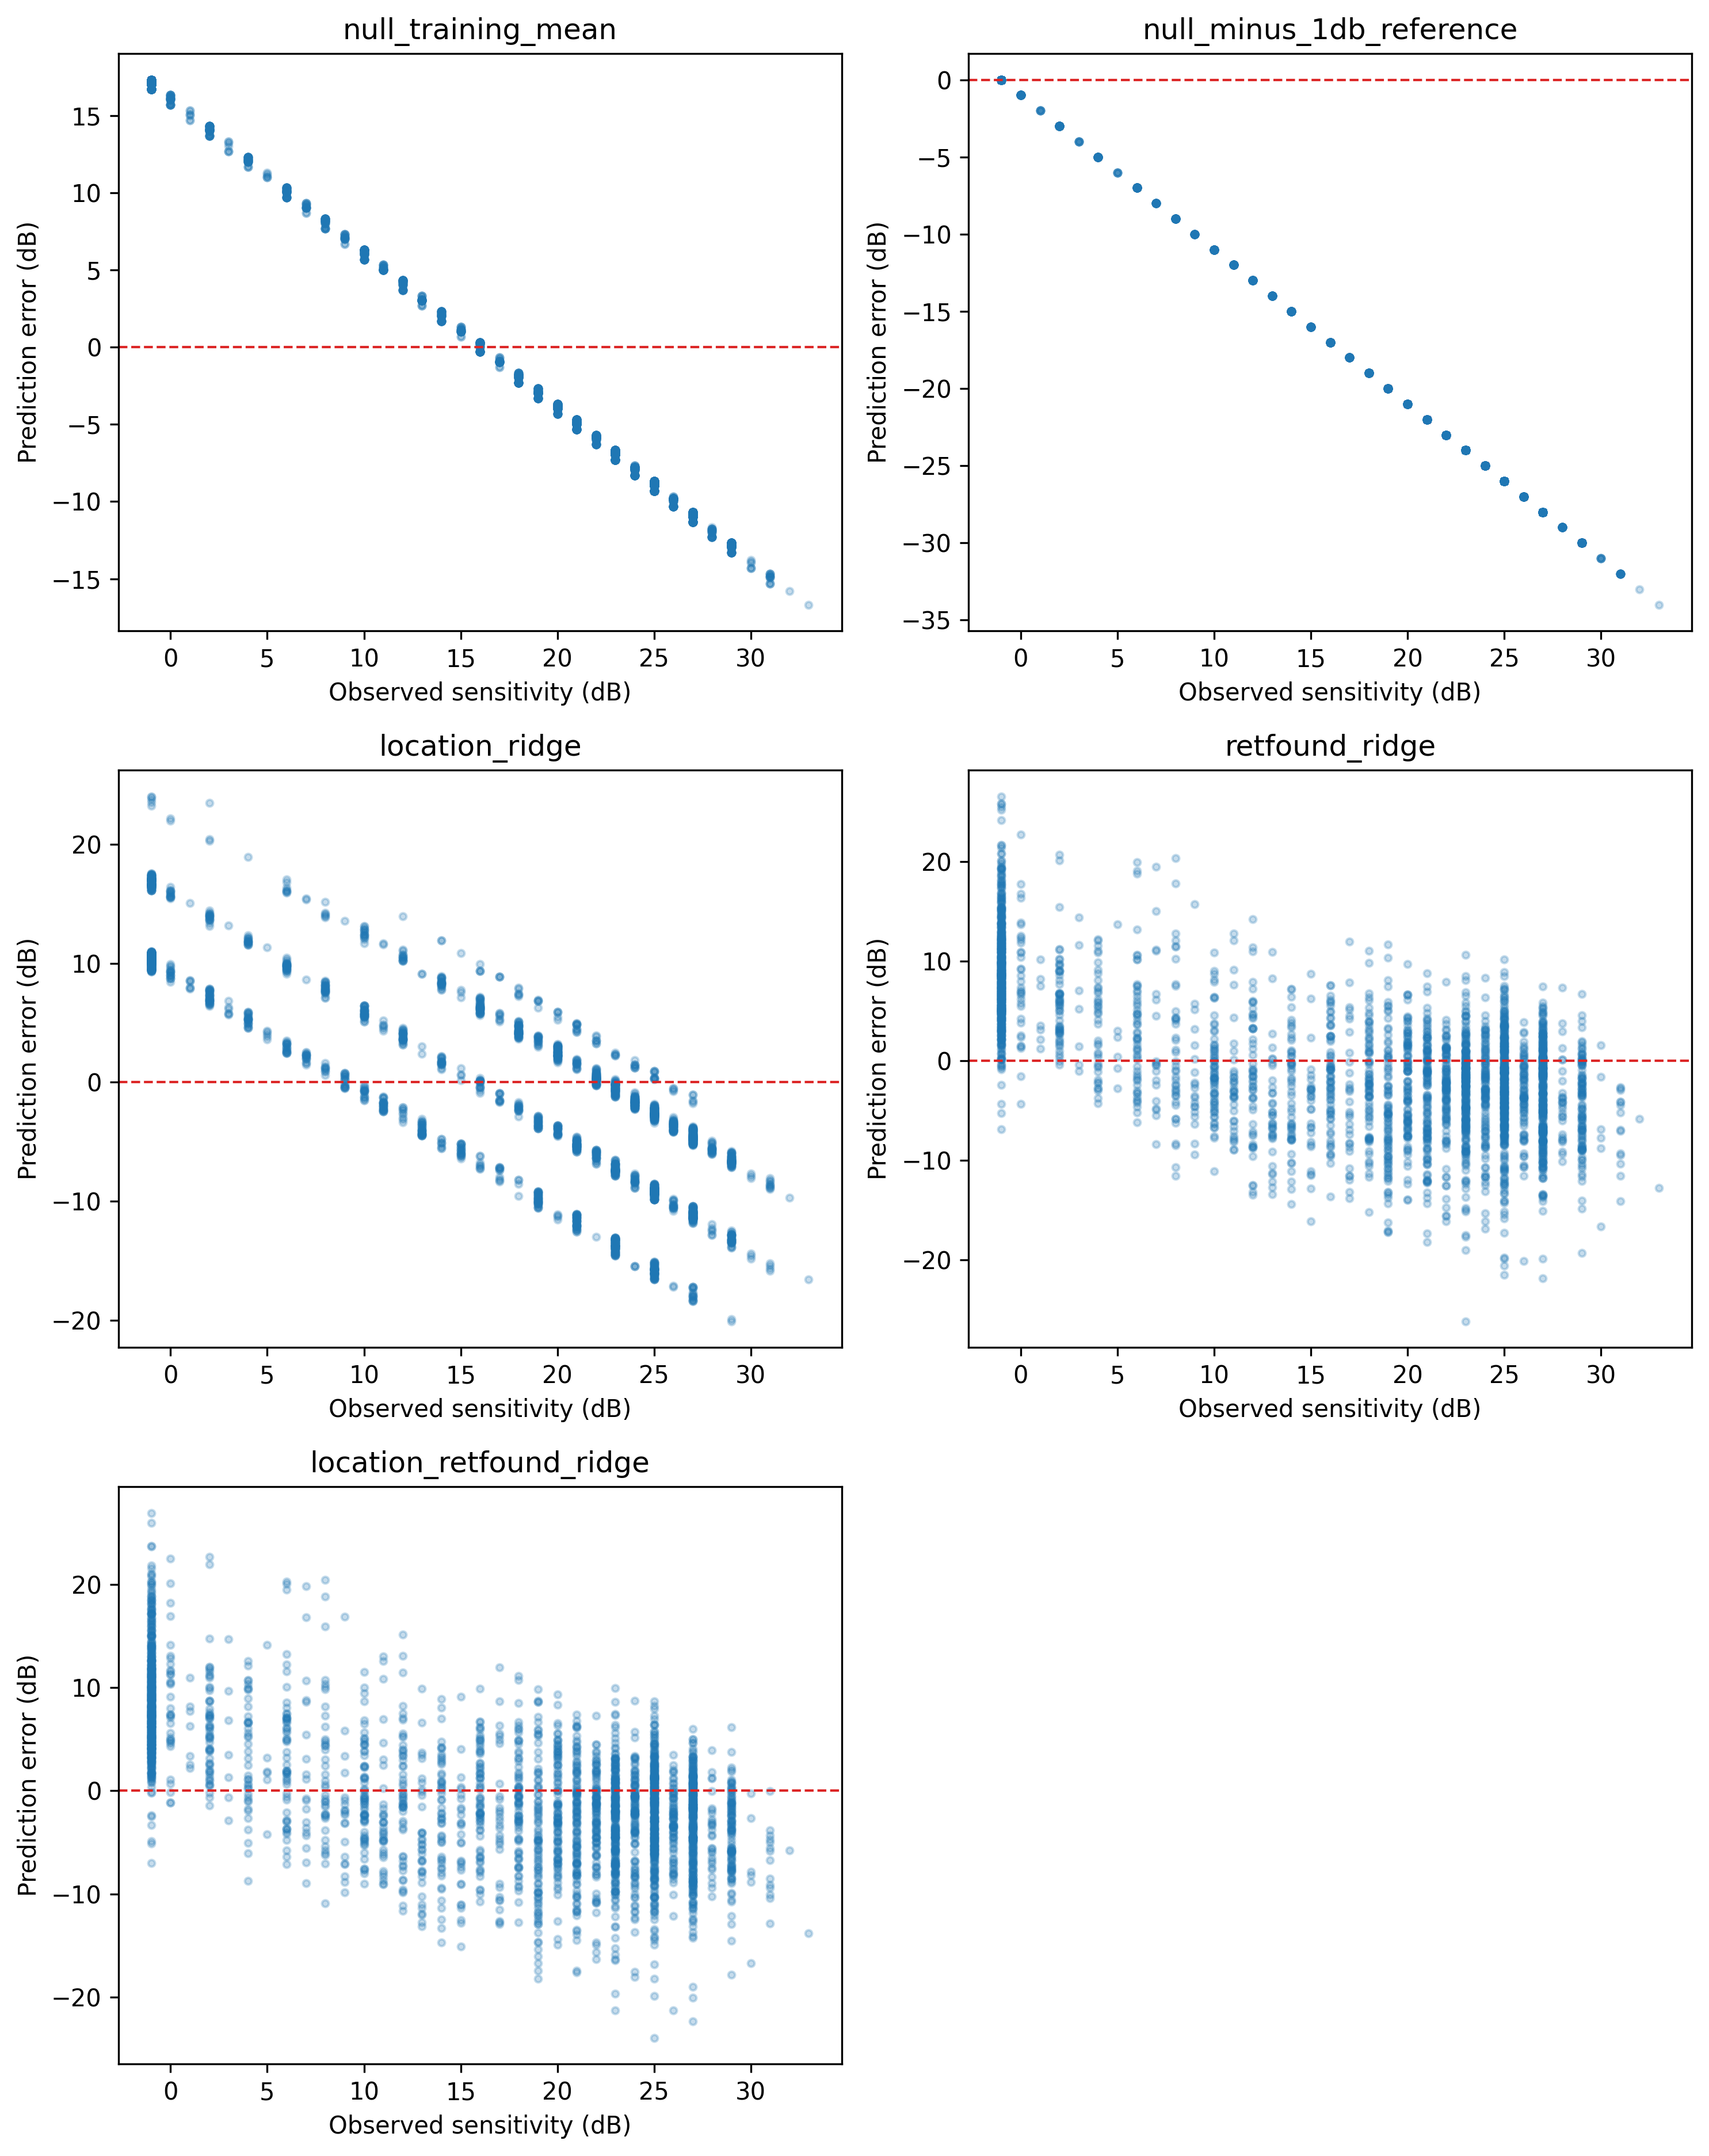
\includegraphics[width=0.98\linewidth]{figure_primary_residual_by_sensitivity.png}
  \caption{Primary residuals stratified by observed sensitivity. The error structure is less favourable at the device floor and at the lowest sensitivities.}
  \label{fig:primary-residuals}
\end{figure}

\begin{figure}[htbp]
  \centering
  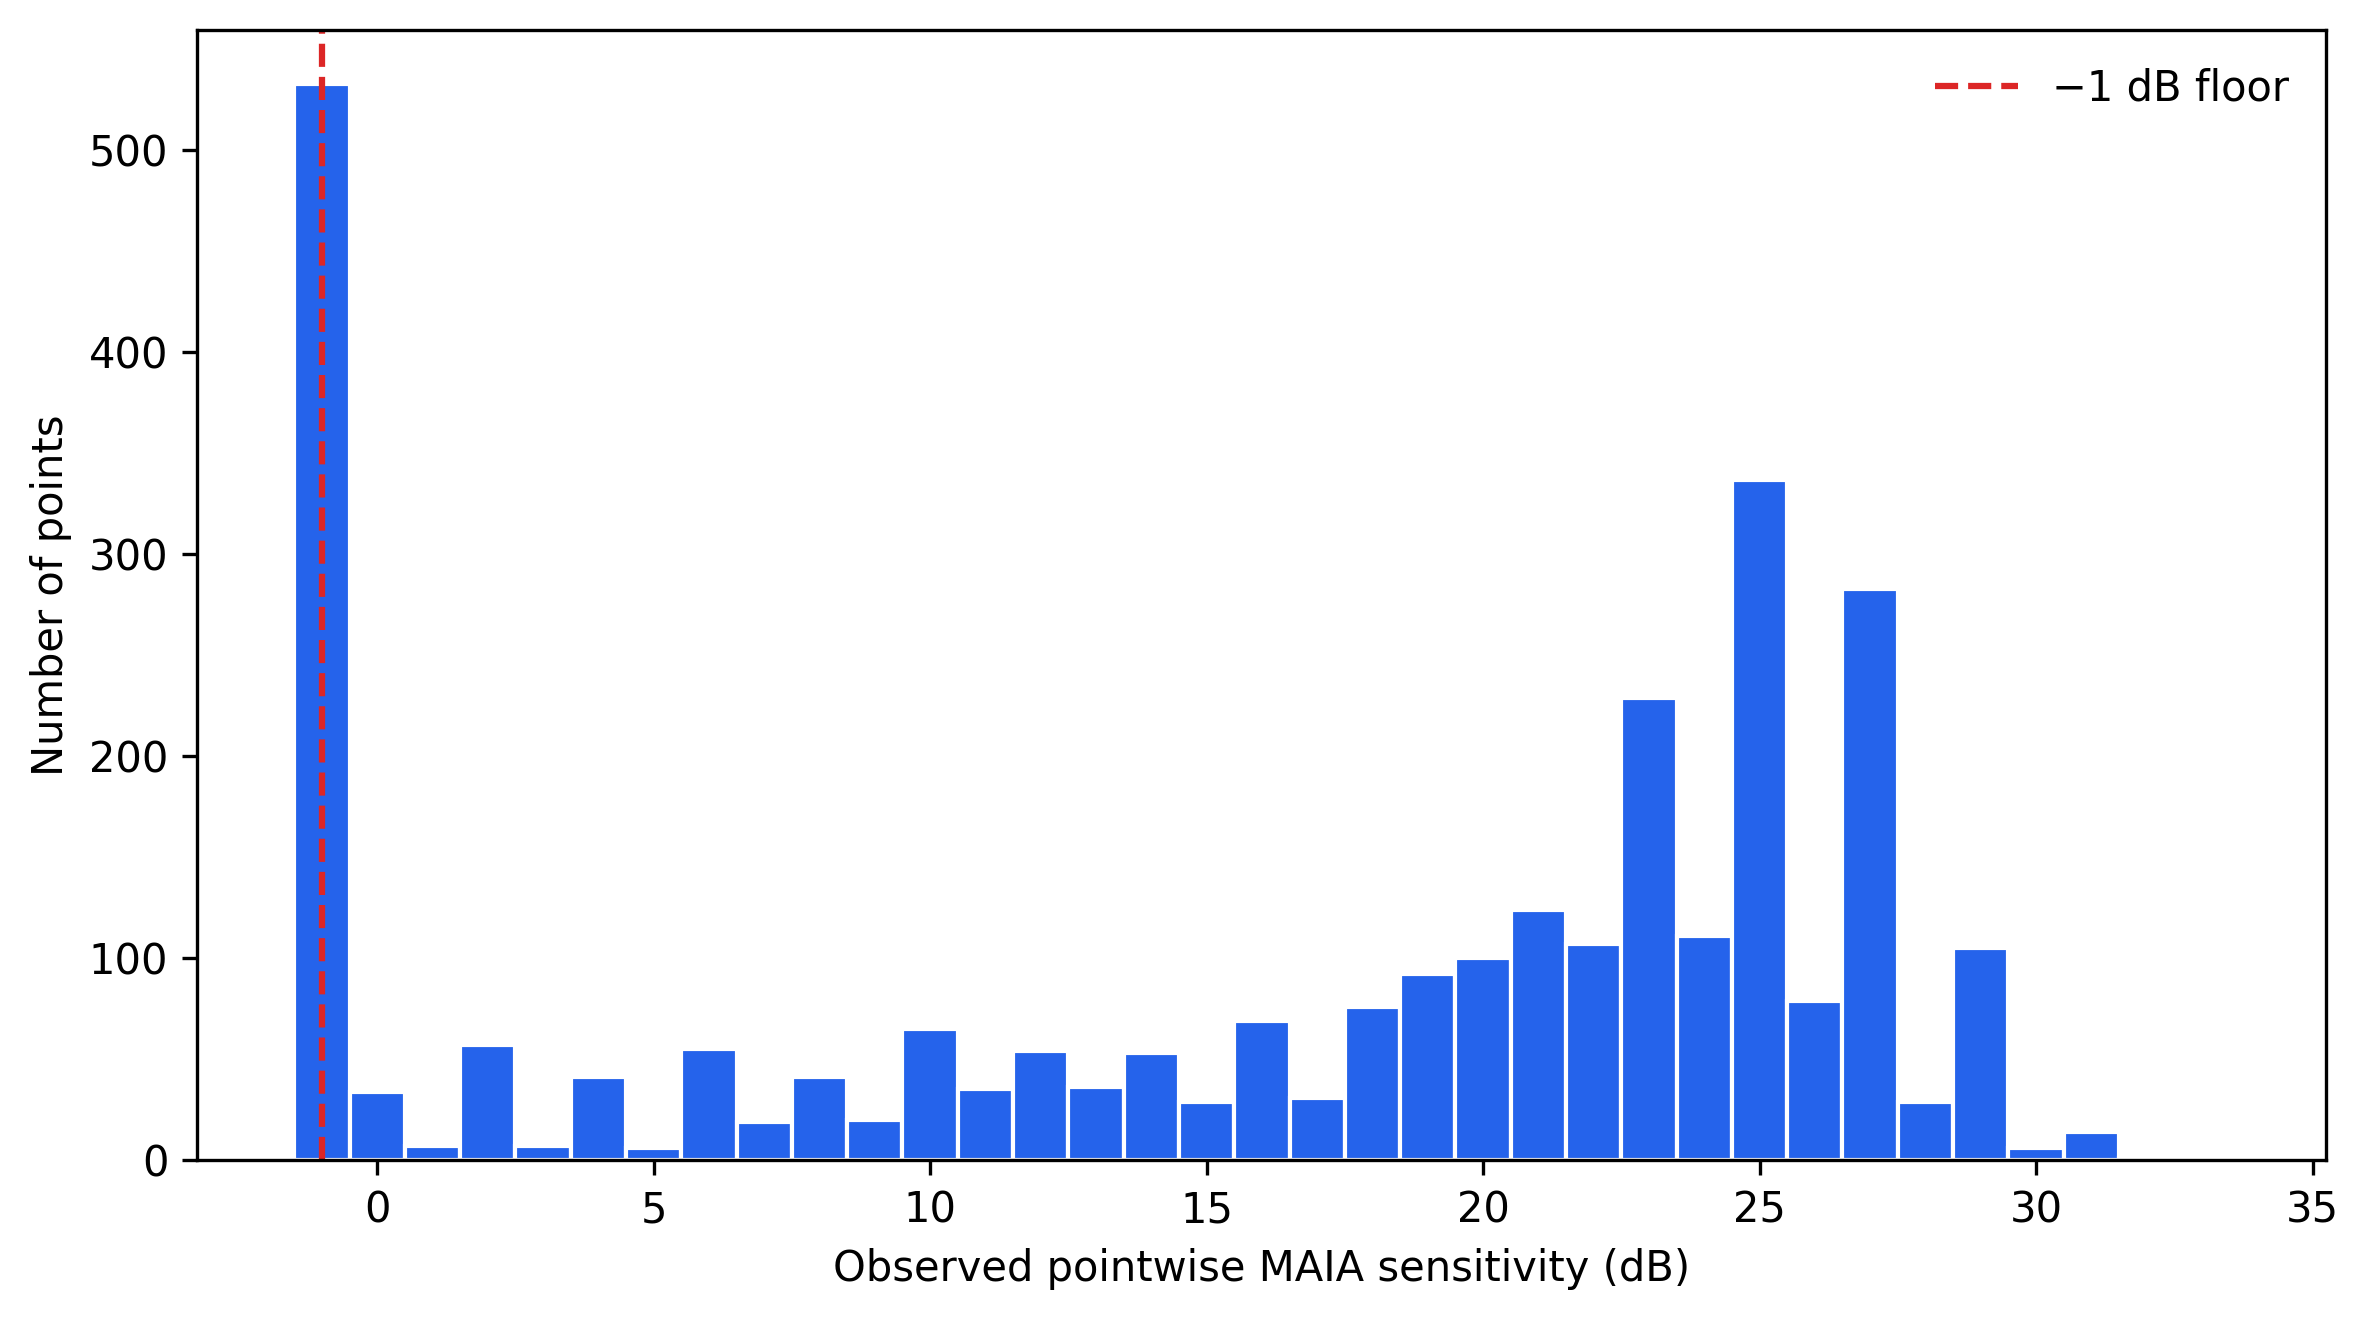
\includegraphics[width=0.85\linewidth]{figure_primary_sensitivity_distribution.png}
  \caption{Distribution of observed pointwise MAIA sensitivity in the primary cohort, including the retained $-1$~dB device-floor observations.}
  \label{fig:primary-sensitivity-distribution}
\end{figure}

\section{Secondary boundary-informed analysis}
\label{sec:secondary-results}

The secondary analysis included the boundary-available subset of 22 participants, 50 eye-visits and 1,850 points. It comprised 13 baseline eye-visits (481 points) and 37 year-one eye-visits (1,369 points), with 278 observations recorded at the $-1$~dB floor. Results from this subset are presented separately because the boundary information was unavailable for the remaining primary-cohort eye-visits.

The location-plus-boundary random forest had the lowest MAE in this analysis at 5.054~dB, with an RMSE of 6.540~dB, bias of $-0.626$~dB, limits of agreement from $-13.390$ to 12.137~dB and supplementary $R^2$ of 0.587. The boundary-aligned RETFound ridge had a similar MAE of 5.114~dB and a lower RMSE of 6.421~dB, while its supplementary $R^2$ was 0.602. The location-plus-boundary RETFound fusion achieved an MAE of 5.577~dB.

\begin{table}[htbp]
\centering
\footnotesize
\caption{Secondary boundary-available out-of-fold performance (22 participants, 50 eye-visits and 1,850 points). B0--B4 are neutral source-mapped boundary labels; $R^2$ is supplementary.}
\label{tab:secondary-performance}
\renewcommand{\arraystretch}{1.12}
\setlength{\tabcolsep}{3pt}
\begin{tabular}{@{}>{\raggedright\arraybackslash}p{0.22\textwidth}>{\centering\arraybackslash}p{0.18\textwidth}>{\centering\arraybackslash}p{0.11\textwidth}>{\centering\arraybackslash}p{0.13\textwidth}>{\centering\arraybackslash}p{0.19\textwidth}>{\centering\arraybackslash}p{0.08\textwidth}@{}}
\toprule
Model & \shortstack{MAE,\\dB} & \shortstack{RMSE,\\dB} & \shortstack{Bias,\\dB} & \shortstack{95\% limits of\\agreement, dB} & $R^2$ \\
\midrule
Training-mean null & 8.700 & 10.207 & $-0.005$ & $-20.016$ to 20.007 & $-0.006$ \\
Fixed $-1$~dB reference & 18.475 & 21.093 & $-18.475$ & $-38.430$ to 1.481 & $-3.294$ \\
Location-only ridge & 7.236 & 8.718 & $-0.005$ & $-17.097$ to 17.088 & 0.266 \\
Boundary-only linear regression & 6.718 & 8.236 & $-0.700$ & $-16.788$ to 15.388 & 0.345 \\
Boundary-only ridge & 6.764 & 8.323 & $-0.661$ & $-16.926$ to 15.605 & 0.331 \\
Location-plus-boundary ridge & 6.623 & 8.169 & $-0.829$ & $-16.762$ to 15.103 & 0.356 \\
Location-plus-boundary random forest & 5.054 & 6.540 & $-0.626$ & $-13.390$ to 12.137 & 0.587 \\
Boundary-aligned RETFound ridge & 5.114 & 6.421 & 0.112 & $-12.475$ to 12.698 & 0.602 \\
Location-plus-boundary RETFound ridge & 5.577 & 6.958 & $-0.672$ & $-14.249$ to 12.905 & 0.533 \\
\bottomrule
\end{tabular}
\end{table}

Figure~\ref{fig:secondary-model-comparison} shows that the secondary ladder has a different ordering from the primary ladder. The location-plus-boundary random forest has the lowest MAE, followed closely by the boundary-aligned RETFound ridge. Both are separated from the training-mean and fixed-reference models, while the linear and ridge models based on boundary features occupy an intermediate range. The error bars for the stronger fitted models overlap, so the figure is most useful for showing the overall model grouping and the small numerical separation between the two best secondary models.

\begin{figure}[htbp]
  \centering
  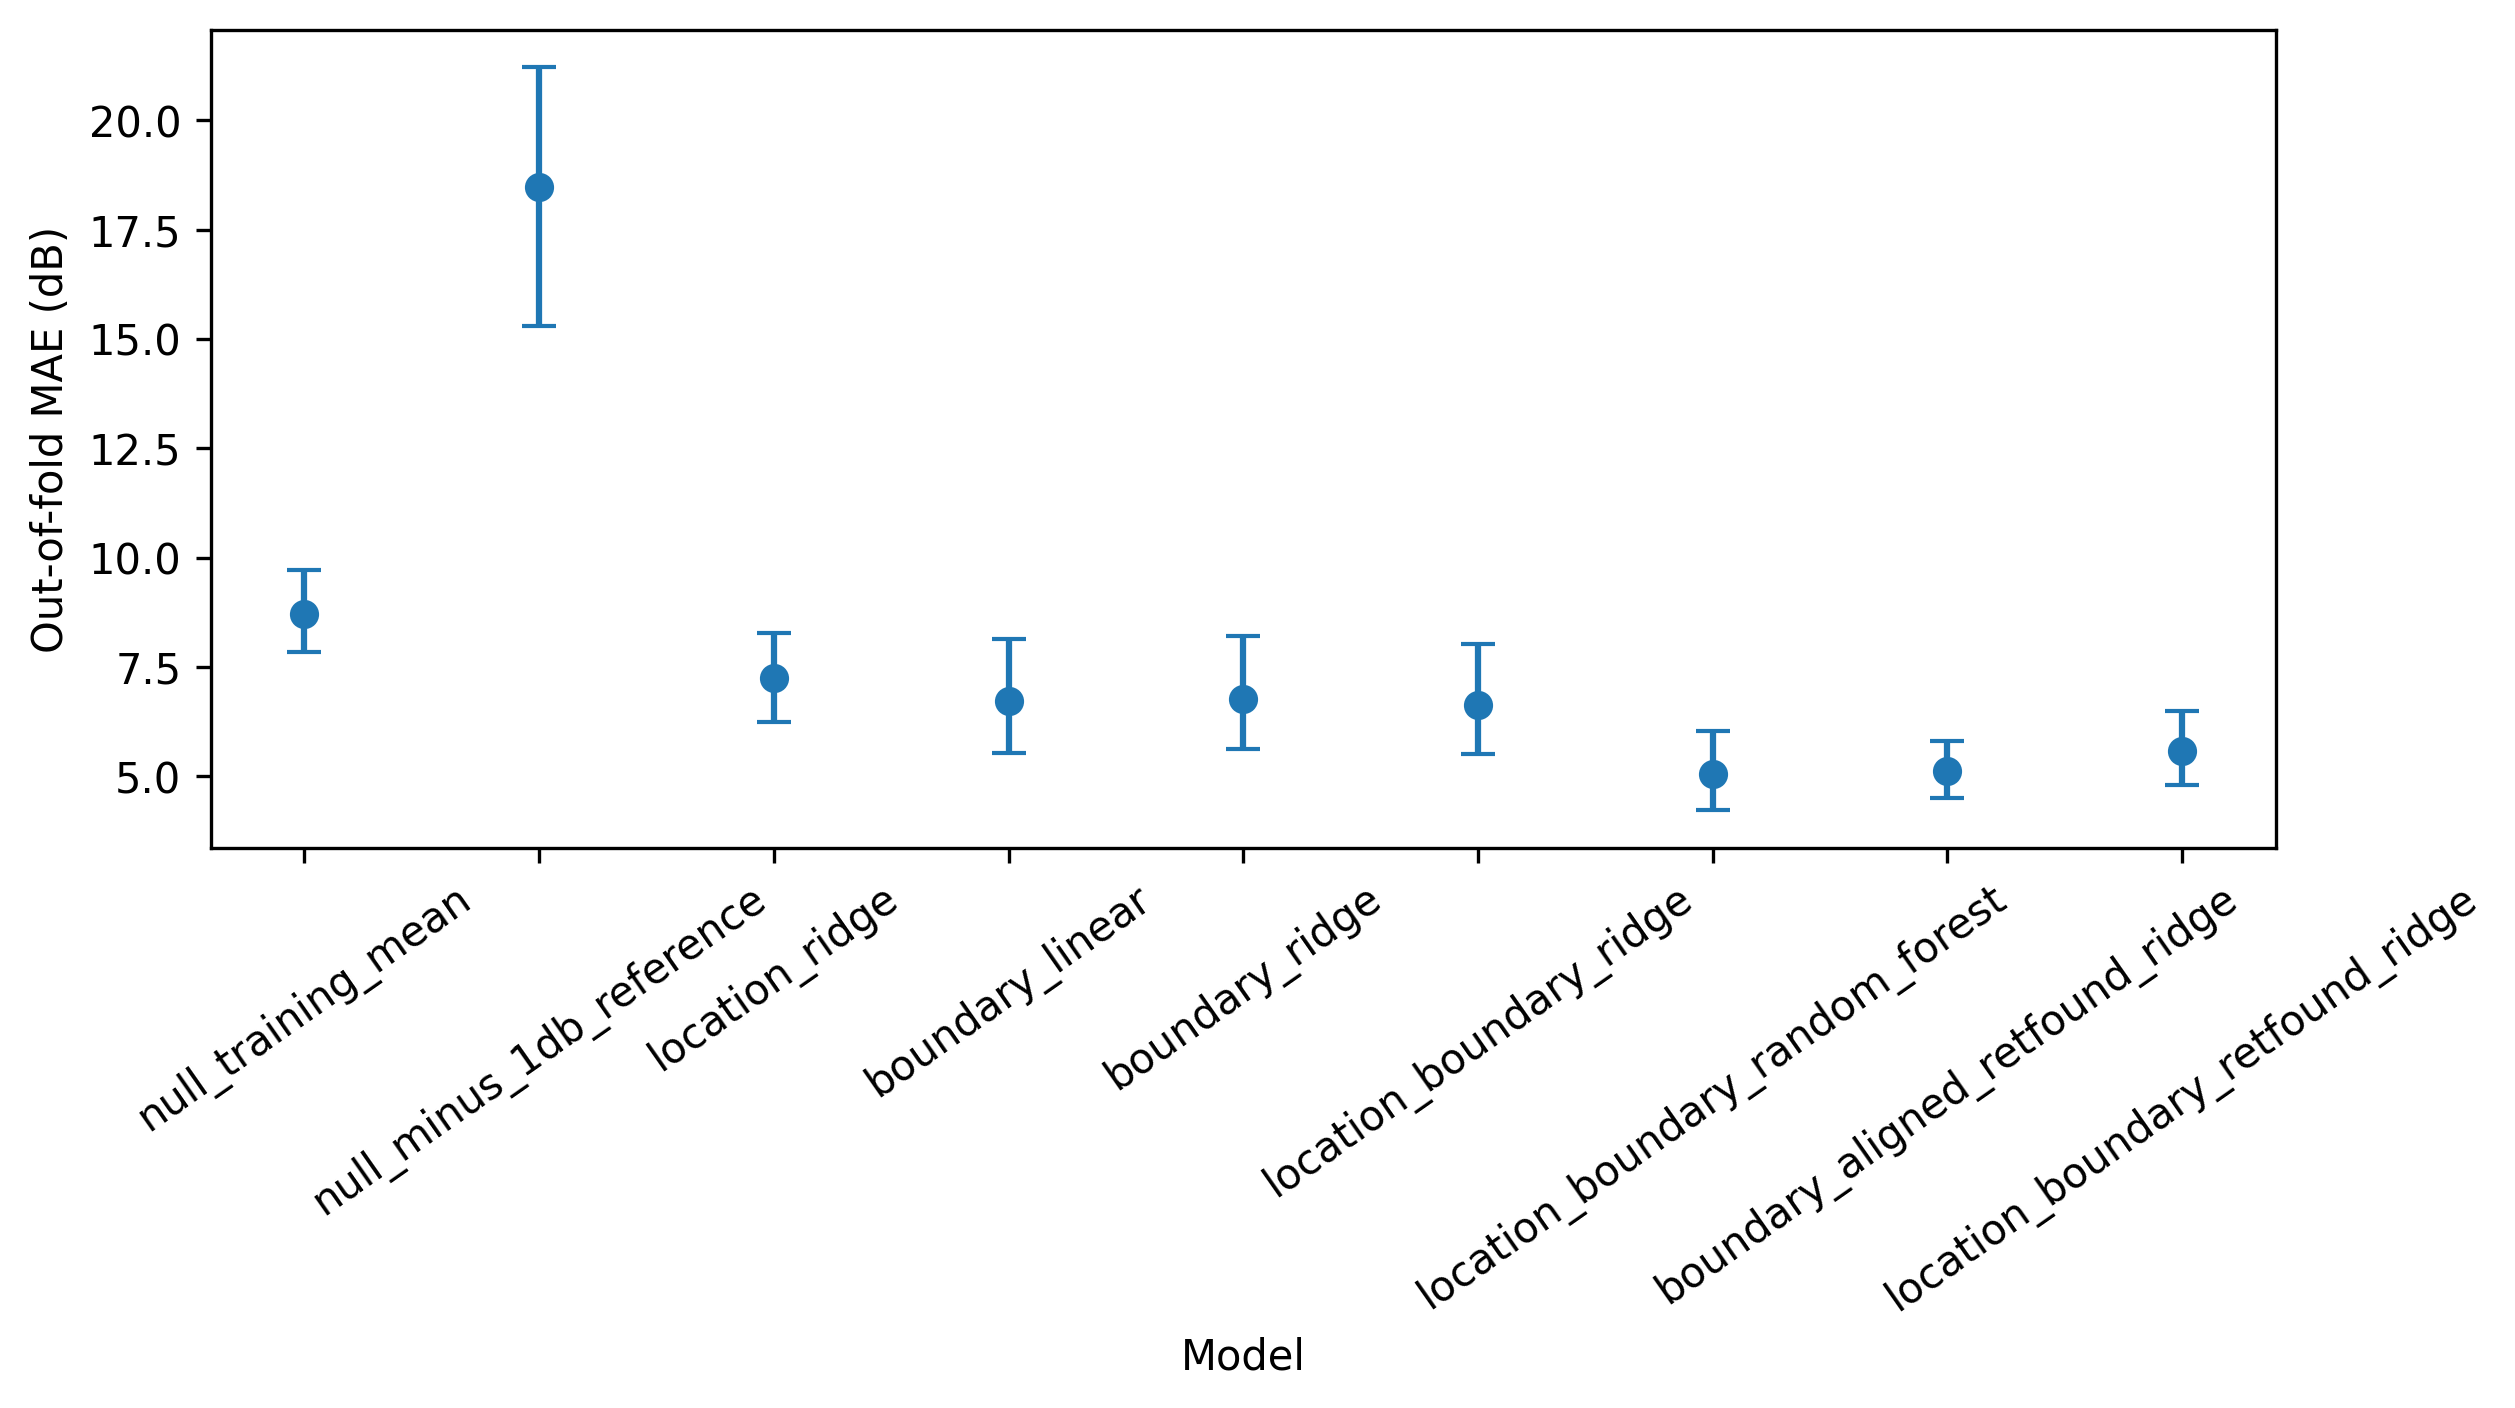
\includegraphics[width=0.95\linewidth]{figure_secondary_model_comparison.png}
  \caption{Model comparison for the boundary-available secondary analysis. The random forest is the best model in this restricted subset by MAE.}
  \label{fig:secondary-model-comparison}
\end{figure}

\begin{figure}[htbp]
  \centering
  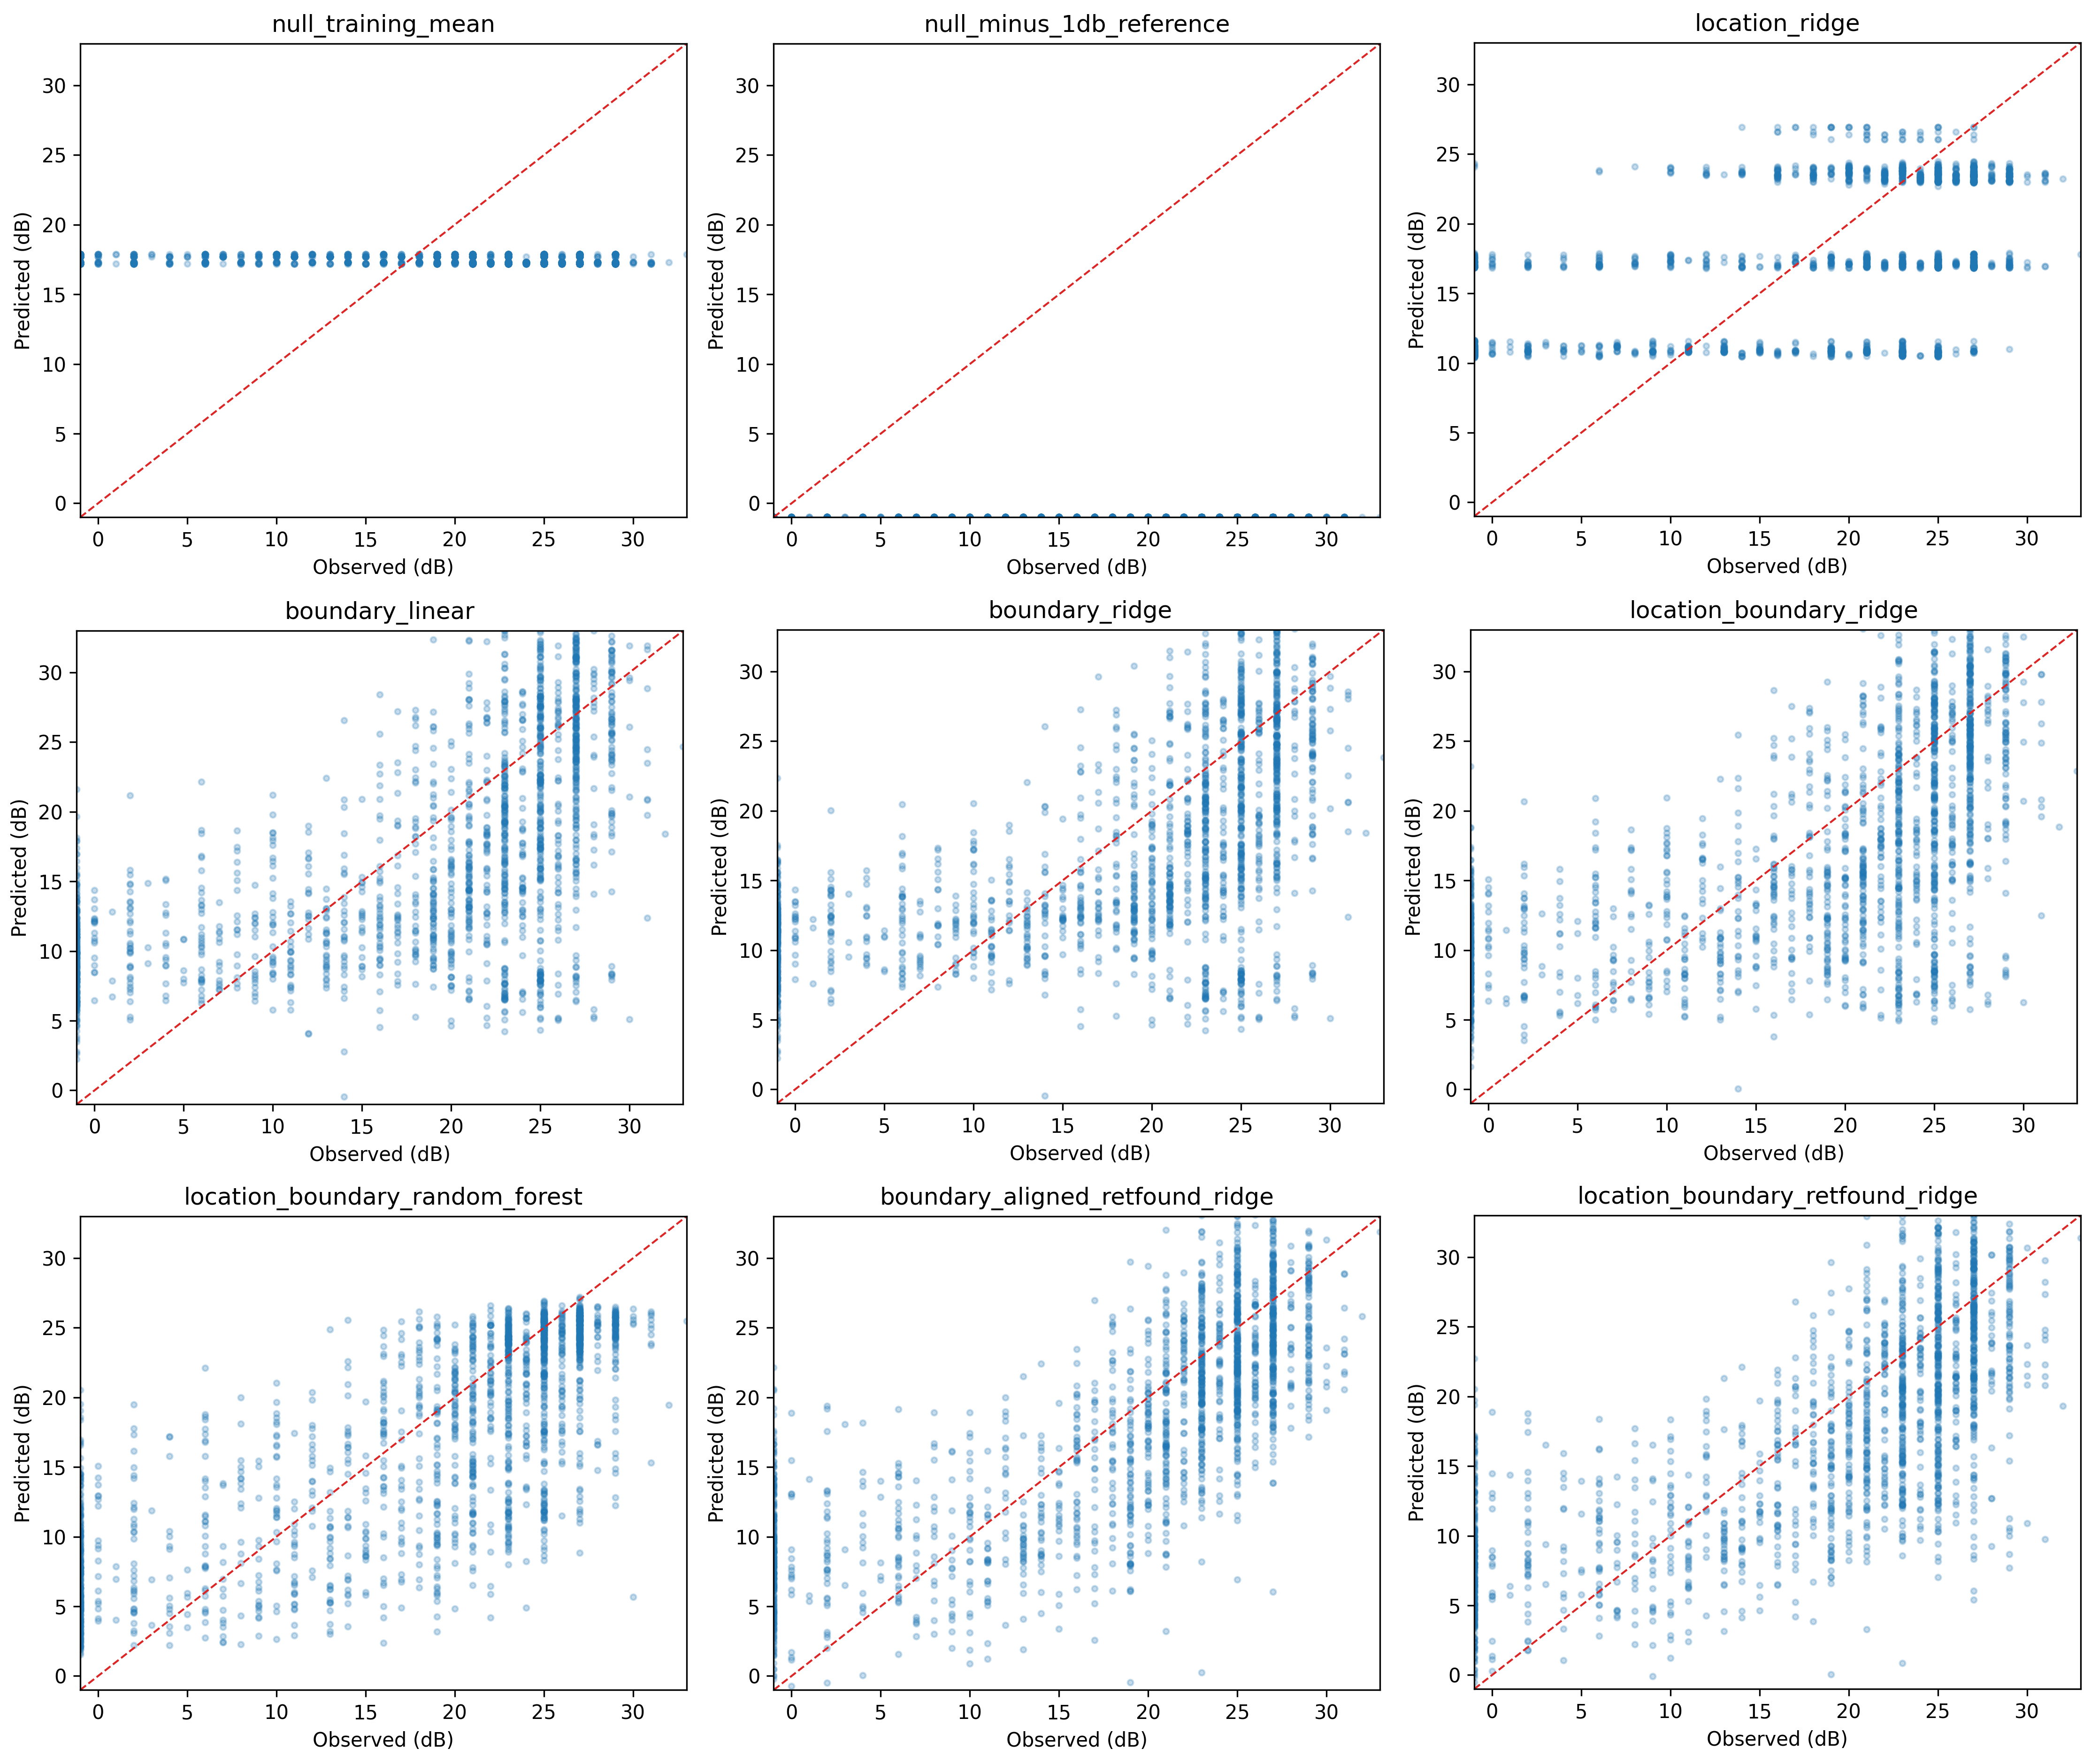
\includegraphics[width=0.99\linewidth]{figure_secondary_observed_predicted_readable.png}
  \caption{Observed versus out-of-fold predicted sensitivity for the nine-model secondary boundary analysis.}
  \label{fig:secondary-observed-predicted}
\end{figure}

The observed-versus-predicted panels in Figure~\ref{fig:secondary-observed-predicted} show a similar progression from constant references to models that vary with the recorded sensitivity. The boundary-only linear and ridge models reproduce some of the observed range but retain a large amount of vertical scatter. The random forest and boundary-aligned RETFound models show a more concentrated association with the diagonal line, particularly through the middle and upper sensitivity range. The fusion model remains variable despite including all three predictor blocks. As in the primary analysis, the panels show repeated values at the lower boundary of the outcome range rather than a continuous spread below the device floor.

\begin{figure}[htbp]
  \centering
  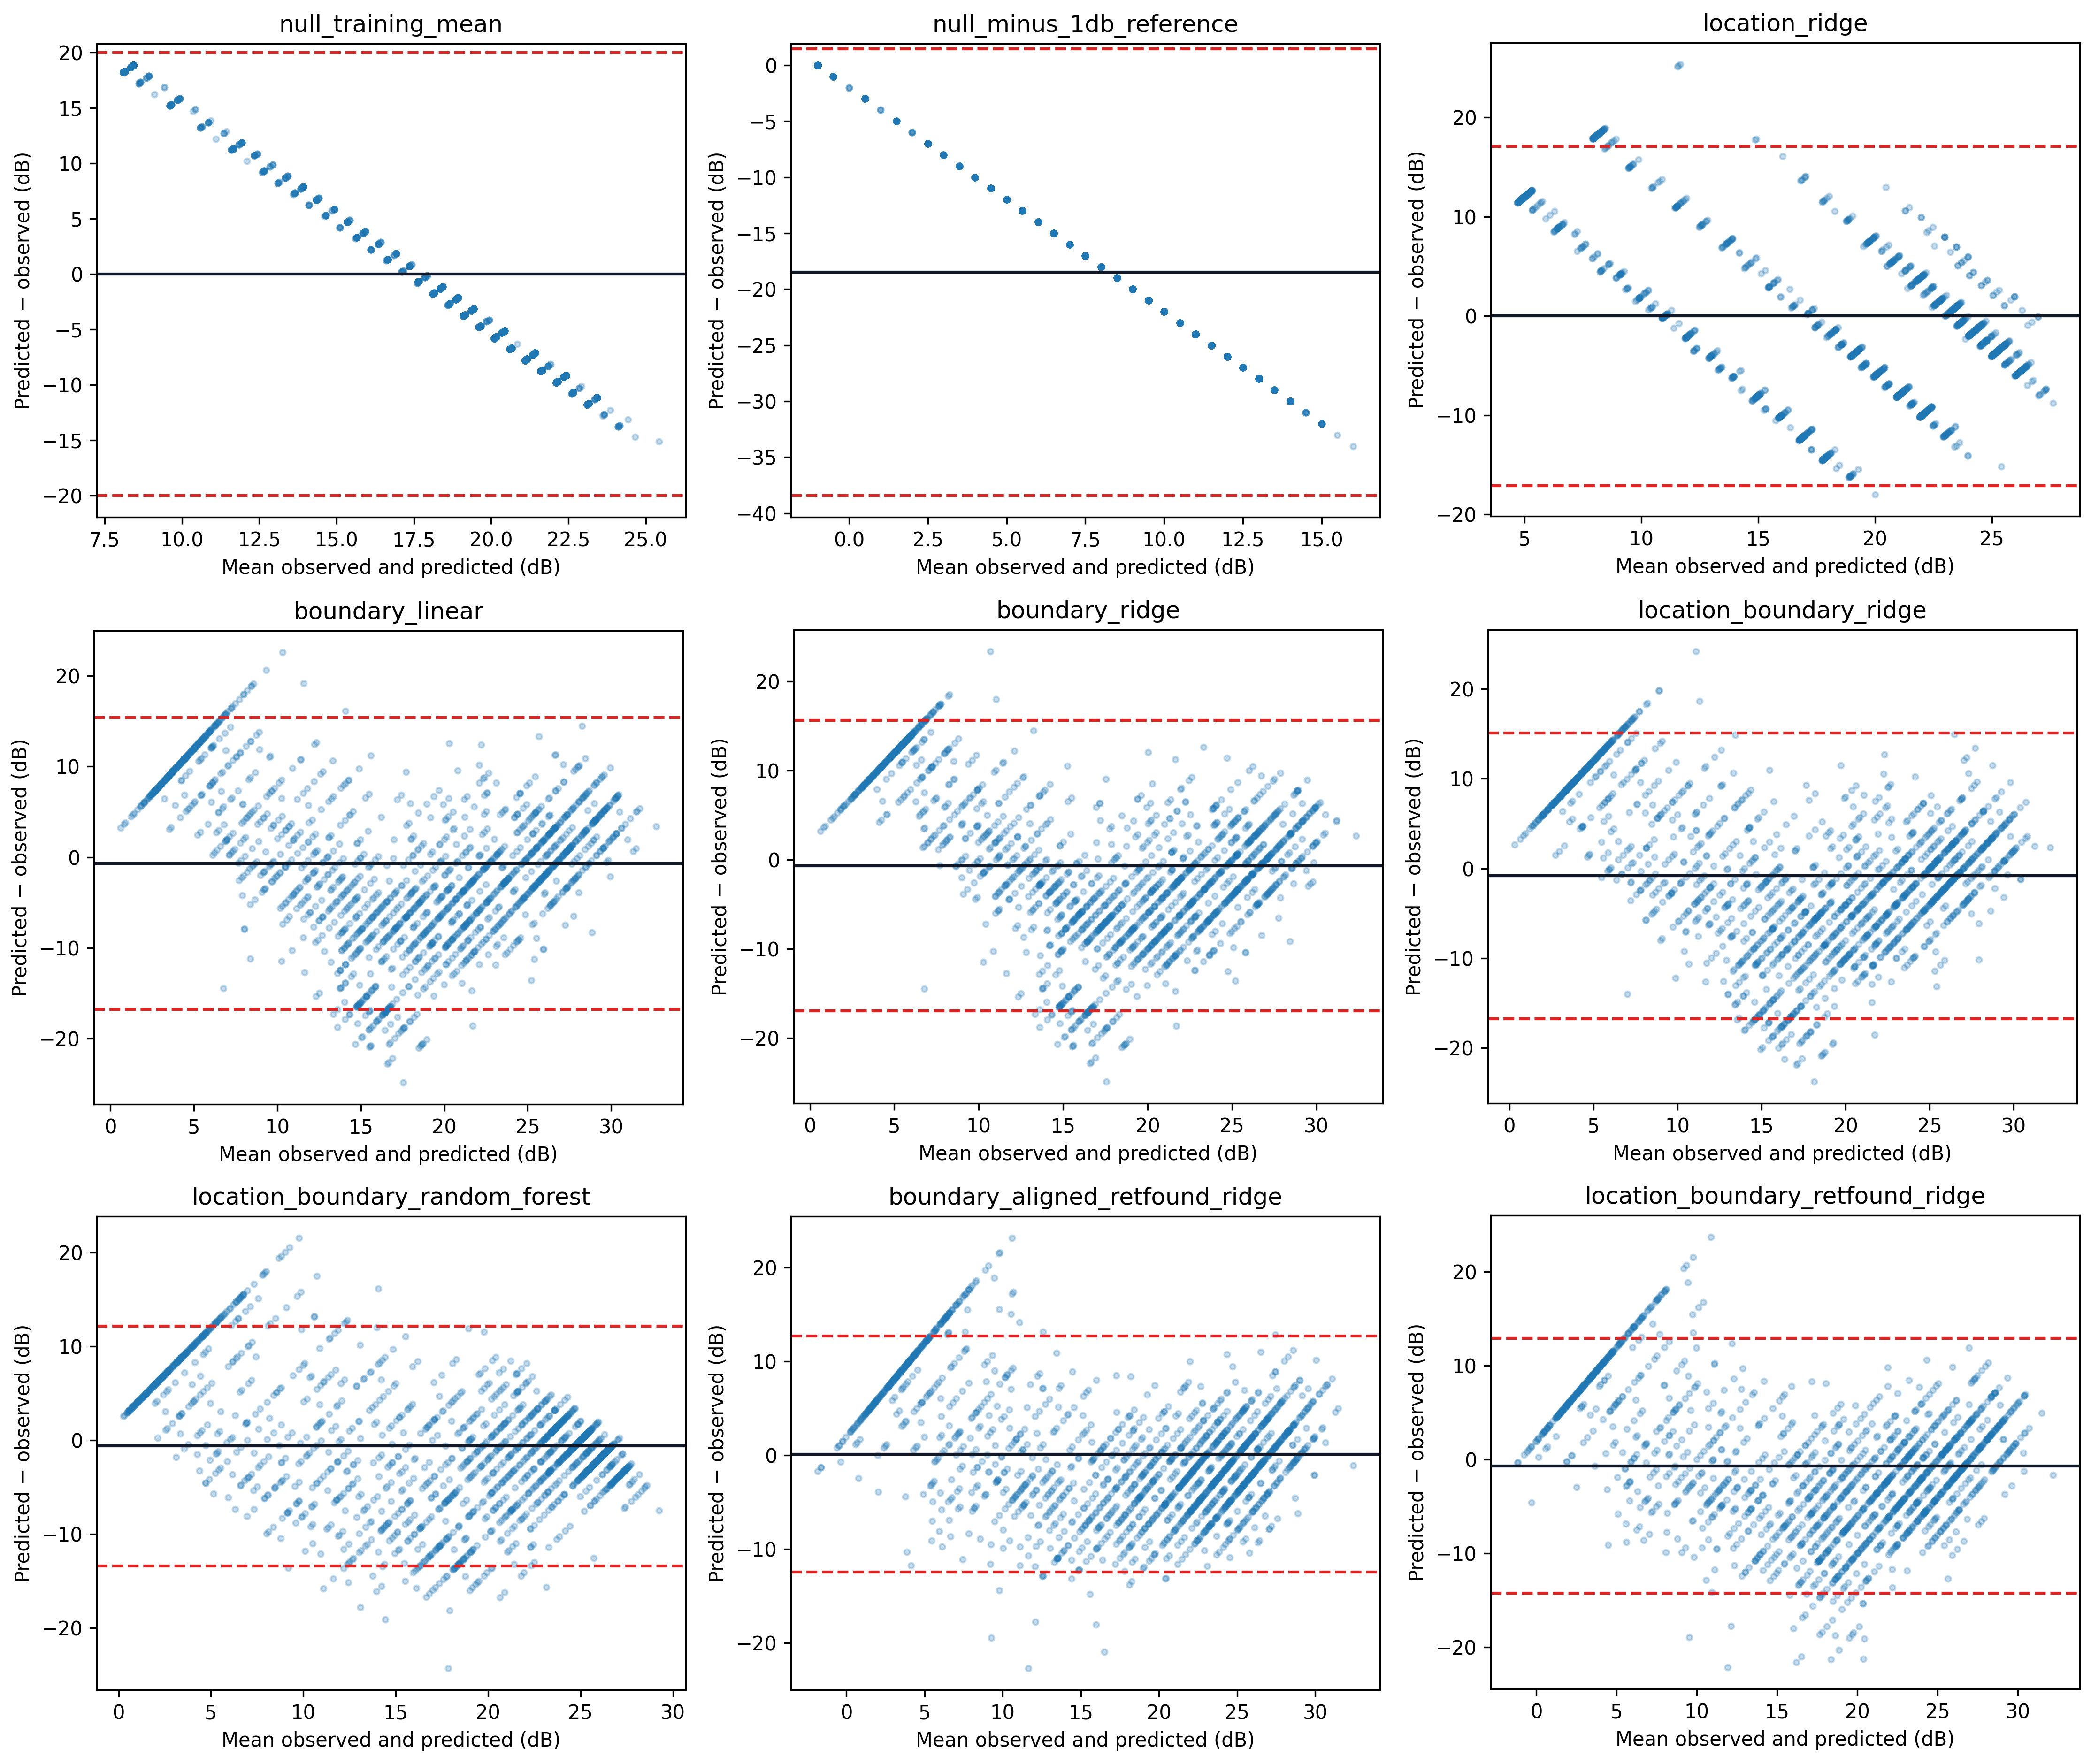
\includegraphics[width=0.99\linewidth]{figure_secondary_bland_altman_readable.png}
  \caption{Bland--Altman plots for the secondary boundary-informed models.}
  \label{fig:secondary-bland-altman}
\end{figure}

The Bland--Altman panels in Figure~\ref{fig:secondary-bland-altman} provide a final view of these secondary differences. The random forest has a modest negative mean bias, whereas the boundary-aligned RETFound ridge is visually more centred around the zero-difference line, which is reflected in its bias of 0.112~dB. Both still show a broad range of pointwise residuals, and the fusion model does not narrow this spread. These plots are descriptive of the boundary-available subset and are presented alongside Table~\ref{tab:secondary-performance}; they are not used to compare this restricted cohort directly with the primary full-cohort analysis.

\chapter{Discussion}
\label{chap:discussion}

\section{Interpretation of the primary findings}

This thesis examined whether local OCT information, once spatially aligned with fundus-controlled microperimetry, could estimate pointwise retinal sensitivity for participants with Usher syndrome who were not used to train the model. The primary results provide evidence that it can contribute useful information in this cohort. The location-plus-RETFound ridge achieved an out-of-fold MAE of 5.485~dB, compared with 7.650~dB for the location-only model and 9.346~dB for the training-mean reference. OCT-derived information was therefore associated with a 2.165~dB reduction in average absolute error beyond what could be obtained from retinal position alone. This is important because retinal position is itself informative in a degenerative retinal disease: a model that only learned that central and peripheral test locations tend to have different sensitivities could appear useful without learning any local structural relationship.

The remaining metrics support a cautious but positive interpretation. The primary combined model had an RMSE of 6.986~dB, a calibration slope of 0.978 and a mean bias of $-0.060$~dB. Its predictions were therefore not systematically shifted above or below the observed sensitivities across the cohort. At the same time, the 95\% limits of agreement extended from $-13.754$ to 13.634~dB. This range shows that individual point estimates can differ substantially from the recorded MAIA value even when the average bias is close to zero. The model should consequently be understood as an internally validated estimate of a structure--function relationship, not as an interchangeable substitute for a microperimetry measurement.

The results also demonstrate why several measures are needed. The supplementary $R^2$ of 0.564 indicates that the out-of-fold predictions captured a meaningful proportion of variation in the recorded endpoint, while MAE describes the typical size of an error on the dB scale. Bland--Altman agreement adds a different perspective by showing the range of error that could occur for an individual point. Taken together, these findings support the conclusion that the local OCT representation contains information about pointwise sensitivity in this cohort, but that this information is not sufficient to make highly precise predictions for every retinal location.

\section{Local OCT context and the effect of within-footprint pooling}

The spatial design was central to this result. A MAIA sensitivity value is produced by a stimulus with an approximately 100~$\mu$m diameter, whereas an OCT volume contains a much denser and wider set of structural measurements. Registration alone does not solve this difference in scale. The image input also has to remain connected to the retinal area represented by the functional test, which is why the three nearest B-scans and the native anchor within the stimulus footprint were defined geometrically before sensitivity was introduced.

Several A-scan positions within the physical footprint were explored during development in an attempt to represent the stimulus area more completely. In the final analyses, this within-footprint pooling was not retained because combining several nearby positions created smoother representations and produced poorer held-out performance than a single centred native anchor on each B-scan. A reasonable interpretation is that neighbouring positions can contain local structural variation that remains relevant to a pointwise endpoint; averaging them can therefore reduce the contrast between a transition region and its surroundings. This is an empirical finding from the present cohort rather than a claim that image pooling is generally inappropriate.

It is also important to distinguish this choice from the use of three B-scans. The final representation still combined the embeddings from the three nearest B-scans, using their mean and population standard deviation, because these were three immediately neighbouring cross-sectional views of the same registered functional location. Pooling across nearby positions along a single B-scan and combining these neighbouring B-scan views answer different questions. The former broadened the local anchor within the stimulus footprint and was less favourable in this study, while the latter reduced dependence on any one cross-section and retained information about variation between scans. This distinction allows the model input to remain local without treating one A-scan as a complete biological description of the stimulus area.

The primary 750~$\mu$m context crop should be interpreted in the same way. It provided surrounding retinal structure to the encoder, but its centre was fixed by the single footprint-aware anchor. The larger visual context therefore did not redefine the functional target. It allowed the representation to include neighbouring morphology that may help place a local structural change within its retinal setting, while the geometric selection rule preserved the link between the target and the OCT input.

\section{Relationship to previous structure--function studies}

The findings are consistent with the broader biological pattern described in Chapter~\ref{chap:background}: preservation of outer-retinal structure is associated with better visual function in inherited retinal disease, although the strength and form of this relationship depend on the clinical endpoint and disease stage. In the baseline RUSH2A analysis, larger ellipsoid-zone area and central retinal thickness were associated with better mean microperimetric sensitivity in participants with \textit{USH2A}-related retinal degeneration \citep{Lad2022}. The later longitudinal RUSH2A study likewise found change in OCT measures and microperimetry over four years, including a decline in mean sensitivity and in sensitivity measured at functional transition points \citep{Vincent2025}. These studies make the present result biologically plausible, but they examine cohort-level or longitudinal associations rather than an image-based prediction for each point in participants held out from training.

There is also a useful distinction between the current result and the numerical values reported in other retinal prediction studies. In geographic atrophy, Pfau et al. reported an imaging-only MAE of 4.64~dB and a lower error after patient-specific calibration \citep{Pfau2020}. Kihara et al. reported an MAE of 3.36~dB for local OCT patches in Macular Telangiectasia type 2 \citep{Kihara2019}. These studies show that structural imaging can support functional estimation, but their errors are not direct targets for this thesis. They used different diseases, functional ranges, image inputs, sampling strategies and, in some cases, data from the participant being predicted. In particular, patient-specific calibration addresses a different clinical and statistical question from prediction for a wholly unseen participant.

The most relevant comparison is therefore the analytical standard rather than the headline MAE. The present work evaluates a pointwise target within a small Usher syndrome cohort, uses an explicitly registered local input and keeps all observations from a participant together during validation. This is more demanding than a random split of retinal points because fellow eyes, repeated visits and nearby points cannot appear on both sides of the split. It is also why the result should not be weakened simply because it is less numerically favourable than values reported in conditions with different data structures. Conversely, a favourable internally held-out result does not establish transportability to another device, site or Usher syndrome subgroup.

The pointwise nature of the endpoint provides further context. Microperimetry is well suited to mapping local function, but it is a psychophysical test and individual points have greater test--retest variability than an eye-level mean. The REPEAT study in retinitis pigmentosa reported pointwise coefficients of repeatability of approximately 8.6--10.2~dB, compared with lower variability for mean sensitivity \citep{Karuntu2025}. Those values cannot be used as a direct threshold for this cohort or for a model prediction, since the study population and test protocol differ. They do, however, show why a 5.485~dB MAE should not be interpreted in the same way as an error for average sensitivity, and why repeated functional measurements would be valuable in a future validation study.

\section{What the image-derived signal may represent}

The improvement beyond the location-only model indicates that the image representation was not acting only as a proxy for the fixed MAIA grid. It does not, however, identify one structure that explains sensitivity. The OCT context may encode several related features, including the continuity of reflective outer-retinal bands, local retinal thickness, the sharpness of structural transitions and the wider pattern of degeneration around the point. These are clinically plausible sources of information because photoreceptor preservation is linked to retinal function, but the frozen representation does not provide a direct biological measurement of any one feature \citep{Tao2016,Gill2022}.

This is one reason why the result is best described as image-derived structural information rather than as proof of a particular anatomical mechanism. A point with lower recorded sensitivity may be associated with a local structural change, but it may also sit within a broader area of degeneration that is represented in the surrounding OCT context. Location, disease severity, visit and unmeasured clinical characteristics can all be related. The comparison with the location-only model helps to isolate added value beyond fixed grid position, yet it does not remove every possible source of confounding. A model trained on a larger and more heterogeneous cohort would be needed to test whether the same representation remains informative after these relationships vary more widely.

The choice of a frozen RETFound encoder was helpful in this setting because it allowed a high-dimensional retinal image representation to be used without fitting a large image model on 22 participants. This constraint was not intended to imply that a pre-trained representation is automatically appropriate for Usher syndrome. RETFound was developed and evaluated across retinal imaging tasks, and the literature shows that the transfer of an OCT model to a new disease needs to be tested rather than assumed \citep{Zhou2023RETFound,Loo2022}. In the present study, the observed improvement over both non-imaging references provides that cohort-specific test. It supports the use of the representation for this particular question, while leaving disease-specific adaptation as a question for future work.

The findings also place the role of explicit engineered features in context. The primary representation is less directly interpretable than a manually measured thickness or boundary distance, but it can retain information from the local image that may not be represented by a small set of summary variables. Conversely, the secondary random forest shows that compact structural features can perform well when verified source data are available. The two approaches should therefore be viewed as complementary. Image-derived features can be useful when consistent boundary information is unavailable, while interpretable measurements can help examine more specific structural hypotheses once their anatomical source is clear.

\section{Secondary boundary-informed findings}

The secondary analysis provided a separate view of the structure--function question in the subset for which source-mapped boundary information was available. Within this cohort, the location-plus-boundary random forest achieved the lowest MAE at 5.054~dB. The boundary-aligned RETFound model was close by MAE at 5.114~dB, while it had the lower RMSE of 6.421~dB and the higher supplementary $R^2$ of 0.602. The two models therefore appear to capture related, but not identical, structural information. The random forest can represent non-linear combinations of the local boundary measurements and retinal location, whereas the image model summarises texture and morphology from the boundary-aligned OCT context without assigning names to the source boundaries.

The fusion model did not improve on either of these models, with an MAE of 5.577~dB. This result is informative because adding more representation types does not necessarily add independent signal, particularly in a small participant cohort. Boundary features, boundary-aligned image features and retinal location can be correlated descriptions of the same disease pattern. A larger fused predictor block can then add variability without adding enough new information to improve predictions for unseen participants. The result supports the use of a model ladder in which each additional input is assessed against simpler alternatives, rather than assuming that a combined model must be stronger.

The secondary results must remain separate from the primary model comparison. Although both analyses included 22 participants, the boundary-available subset contained 50 eye-visits and 1,850 points, rather than the 78 eye-visits and 2,886 points in the full cohort. The smaller error in the secondary analysis may consequently reflect differences in eligibility, visit composition or sensitivity distribution as well as the representations and models under consideration. It cannot be interpreted as evidence that boundary features are superior to the full-cohort representation.

The neutral B0--B4 labels also constrain biological interpretation in an appropriate way. The results show that the verified source-derived intervals were useful predictors in this subset; they do not establish that a particular named retinal layer causes a change in sensitivity. Independent confirmation of the anatomical definitions and segmentation provenance would be needed before relating an individual interval to a specific outer-retinal structure. This is particularly relevant in Usher syndrome, where the relation between structural preservation, degeneration stage and measured function may vary across locations and participants \citep{Gill2022,Loo2022}.

\section{Error patterns, strengths and limitations}

The descriptive strata show where the primary model was less and more reliable within the available data. MAE was 8.787~dB for observations recorded at the $-1$~dB MAIA floor, compared with 4.737~dB above the floor. At the floor, several levels of severe functional loss can receive the same recorded value. This reduces the information available to a regression model and makes the observed target less able to distinguish between nearby levels of impairment. It also means that an estimate near the floor cannot be read as a precise measure of residual function. The lower error at year one than at baseline is descriptive only, since the visit groups differed in their numbers of observations and participating individuals.

Several features of the study strengthen the interpretation. OCT and MAIA data were paired at the same visit, and the registration was visually reviewed before pointwise modelling. The primary analysis retained all eligible matched observations rather than restricting the main question to the boundary-available cases. It also used transparent non-imaging references, a constrained representation model and nested participant-grouped validation. These decisions make the reported improvement over location less likely to arise solely from spatial co-location or from correlated observations being shared between the training and test sets.

However, internal validation does not create an external cohort. The number of participants was 22, and the apparently larger number of point rows includes correlations within eyes, visits and participants. Participant-level folds and participant-bootstrap intervals address this clustering during evaluation, but they cannot represent disease diversity that is absent from the data. The models also rely on the quality of the MAIA--OCT/SLO registration, OCT acquisition and MAIA response. A small local misregistration, poor fixation or an unobserved scan artefact can affect an individual prediction even when the overall transform has passed review.

The endpoint itself represents recorded sensitivity, not an error-free latent measure of retinal function. Fatigue, attention, learning effects and disease severity can affect microperimetry, while the device floor creates a censored part of the outcome range \citep{Pfau2021Microperimetry,Karuntu2025}. The present analyses therefore cannot separate all functional measurement variability from structural prediction error. They are also cross-sectional in their main inference: paired baseline and year-one visits contribute observations, but the study was not designed to estimate whether an OCT model detects within-person progression or a response to treatment.

The study also makes no claim about diagnosis. Its endpoint was a continuous sensitivity value at a known retinal location in people already represented within an Usher syndrome cohort. It cannot determine whether an individual has Usher syndrome, distinguish between genetic subtypes, or infer a participant's broader visual experience from a local dB estimate. These boundaries matter because a useful research model can still have a narrow intended use. Keeping that use specific makes it possible to evaluate the model against the appropriate reference---direct functional testing at the corresponding retinal point---instead of attaching wider clinical claims to its performance.

\section{Implications for research and clinical monitoring}

The appropriate implication is not that OCT can replace microperimetry. The wide individual-point agreement limits, the device floor and the absence of external validation rule out that conclusion. Instead, the study provides a reproducible, spatially explicit basis for asking when OCT carries useful information about local function. This could be valuable in research settings where microperimetry is burdensome, where an objective structural complement is needed, or where a future trial wishes to understand whether structural and functional changes move together.

For Usher syndrome studies, this question is increasingly relevant because clinical trials require endpoints that are reliable, sensitive to change and suited to the stage of disease being studied. Recent RUSH2A endpoint work emphasises the difficulty created by slow progression and variation between participants, and recommends that endpoint selection be linked to the capacity to observe change in untreated eyes \citep{Maguire2024}. The present model is not an endpoint proposal, but it suggests that registered local OCT could be investigated alongside direct functional measures rather than treated as a proxy without validation. Any future use should specify the intended decision, the acceptable uncertainty for that decision and the way in which an uncertain or failed prediction would be handled.

There may also be a practical role in supporting the interpretation of incomplete functional data. For example, an image-derived estimate could help describe the structural context of a missing or unreliable MAIA point during a research visit, provided that it is clearly labelled as an estimate rather than treated as an observed response. This would still require external evidence that the model is reliable in the relevant setting. Its value would depend on whether it improves the quality of a research assessment, not simply on whether it produces a plausible number.

Overall, the results support a positive but limited conclusion. Local OCT representations improved held-out prediction of pointwise MAIA sensitivity beyond retinal location in this Usher syndrome cohort. The smaller boundary-informed analysis further showed that source-mapped structural intervals and boundary-aligned image representations each contained useful signal, although their relative performance cannot be compared directly with the primary analysis. The work therefore supports further investigation of OCT-based functional estimation while retaining direct microperimetry as the reference functional measurement.

\chapter{Conclusion}
\label{chap:conclusion}

This thesis developed a reproducible framework for relating pointwise MAIA sensitivity to local OCT information in matched Usher syndrome visits. The framework links the functional and structural modalities through saved registration and quality-control decisions, three-nearest-B-scan mapping, approximately 100~$\mu$m footprint-aware sampling and hierarchical pooling to a point-level representation. It then evaluates prespecified models using participant-grouped nested validation rather than treating neighbouring retinal samples as independent cases.

The primary analysis preserves the all-eligible cohort by using a label-blind RETFound representation; the B0--B4 structural analysis is appropriately secondary and availability-limited. The location-plus-RETFound ridge was the best primary model (MAE 5.485~dB, 95\% CI 4.871--6.177; RMSE 6.986~dB; bias $-0.060$~dB; Bland--Altman limits $-13.754$ to 13.634~dB), improving on the location-only ridge (MAE 7.650~dB) and the training-mean null (9.346~dB). These values must be interpreted alongside the participant-level uncertainty, the device-floor error and the remaining limits of agreement, not in isolation.

The study shows that, within this internally evaluated cohort, spatially aligned local OCT information improves prediction of recorded pointwise sensitivity beyond simple non-imaging references. It does not demonstrate that OCT replaces microperimetry, that a named retinal layer drives function, or that the approach generalises beyond this cohort. Its contribution is an evidence-traceable spatial and statistical framework through which those stronger claims can be tested in future data.

\chapter{Future Work}
\label{chap:future-work}

\section{External and longitudinal validation}

The immediate priority is an external validation study using independently acquired MAIA and OCT data. It should include more than one clinical site where possible and should record scanner type, acquisition protocol and image quality so that any loss of performance can be interpreted. A prospective design would also allow the eligibility criteria, acceptable agreement range, calibration assessment and handling of missing or low-quality examinations to be specified before model evaluation. Such a study should retain participant-level splits and report performance separately across clinically relevant disease stages rather than relying on a pooled point-level result.

Longitudinal data are particularly important. The RUSH2A natural-history studies have shown that both OCT measures and microperimetry change over time, while functional transition-point sensitivity may be responsive to clinically meaningful decline \citep{Vincent2025,Maguire2024}. Future work should therefore test whether image-derived estimates track within-person change across repeated visits, not only cross-sectional differences between retinal points. This will require a model that accounts for repeated measures and for the fact that deterioration may be slow and heterogeneous. Pointwise sensitivity may remain useful, but mean sensitivity and sensitivity at carefully defined transition regions should be evaluated alongside it when the intended use is trial monitoring.

\section{Outcome, uncertainty and spatial representation}

Repeated microperimetry at the same visits would make it possible to model measurement reliability directly. In particular, a future analysis could distinguish observations at the device floor, quantify test--retest variation in the study population and report prediction intervals that combine model uncertainty with outcome variability. This would be more useful than a single MAE when deciding whether an estimate is sufficiently reliable for a particular research task \citep{Pfau2021Microperimetry,Karuntu2025}.

The spatial ablation in this thesis also suggests a focused methodological question. Multiple within-footprint A-scan positions should not simply be averaged because pooling smoothed the local representation and was less effective for the pointwise target in this cohort. With a larger dataset, future work could compare pre-specified alternatives: one centred anchor, learned attention across a small set of anchors, and representations that preserve the distribution of local features without collapsing it into a mean. These comparisons should be conducted within the same participant-grouped validation design. The three-B-scan summary should likewise be tested against explicit models of scan-to-scan variability, while maintaining the link between each OCT input and the MAIA stimulus location.

\section{Boundary data and representation development}

The B0--B4 source should be linked to an authoritative description of the boundary definitions before any named-layer interpretation is attempted. Once this provenance has been verified, a larger boundary-available cohort could compare engineered interval features, segmentation-derived features and boundary-aligned image representations on the same cases. Disease-specific segmentation is likely to be important: an ellipsoid-zone model trained in another disease transferred poorly to \textit{USH2A}-related degeneration until it was retrained on relevant data \citep{Loo2022}. The same principle applies to foundation-model features. RETFound provides a reasonable starting representation, but fine-tuning or further self-supervised adaptation should only be considered with enough independent data to evaluate whether it improves on the current constrained model \citep{Zhou2023RETFound,Gholami2024}.

\section{Path towards clinical use}

Any clinical or trial-facing tool would need to be evaluated as a decision-support intervention rather than only as a prediction model. Its intended user, input requirements, output, uncertainty display and failure cases should be defined in advance, together with evidence that using the output improves a real decision. These are consistent with the reporting priorities set out in CONSORT-AI, including transparent descriptions of inputs, human--AI interaction and error analysis \citep{Liu2020}. Until that evidence is available, the most appropriate role for OCT-based sensitivity estimates is as a research adjunct that complements, rather than replaces, direct functional testing.


\appendix
\renewcommand{\chaptername}{Appendix}
\chapter{Guide to the Accompanying Notebook}
\label{app:reproducibility}

The accompanying public repository contains a sanitised record of the computational workflow used in this thesis. It retains the implementation of data preparation, MAIA--OCT/SLO registration, point-level OCT representation construction, model fitting and evaluation described in Chapter~\ref{chap:methods}. A separate synthetic-data demonstration executes the central participant-grouped modelling and evaluation pattern without clinical inputs.

Clinical data and participant-level outputs are not included. The repository is therefore an inspectable account of the analytical approach and reported outputs rather than a standalone clinical-data package.

\section{Notebook guide}

Table~\ref{tab:notebook-guide} indicates how the main components of the notebook relate to the thesis.

\begin{longtable}{p{0.30\linewidth}p{0.60\linewidth}}
\caption{Guide to the accompanying notebook.}\label{tab:notebook-guide}\\
\toprule
Notebook component & Purpose in the thesis \\
\midrule
\endfirsthead
\toprule
Notebook component & Purpose in the thesis \\
\midrule
\endhead
Data preparation and cohort definition & Creates the de-identified analytical records and applies the eligibility criteria described in Section~\ref{sec:cohort}. \\
MAIA--OCT/SLO registration & Implements the spatial mapping and visual quality-control procedure described in Section~\ref{sec:registration}. \\
Point-level OCT representation & Identifies the local B-scans and constructs the image-derived and boundary-derived predictors described in Sections~\ref{sec:footprint} and~\ref{sec:representations}. \\
Primary and secondary modelling & Fits the prespecified model ladders using participant-grouped validation, as described in Sections~\ref{sec:models} and~\ref{sec:validation}. \\
Evaluation and reporting & Calculates the performance measures and produces the tables and figures used in Chapter~\ref{chap:results}. \\
\bottomrule
\end{longtable}

\chapter{Supplementary Methodological Detail}
\label{app:supplementary-methods}

This appendix provides additional context for the registration, model configuration and diagnostic assessment reported in Chapter~\ref{chap:methods}.

\section{Registration and spatial quality control}

Figure~\ref{fig:supplementary-qc} shows synthetic registration examples. Each panel illustrates the kinds of scale and orientation variation considered during review and provides visual context for the registration procedure described in Section~\ref{sec:registration}.

\section{Model configuration and validation}

The primary and secondary analyses used separate model ladders because their OCT predictor representations were different. The primary analysis used image-derived representations for the full eligible cohort, whereas the secondary analysis used source-mapped boundary features in the restricted boundary-available cohort. Both analyses retained participant-grouped validation and training-only preprocessing, as described in Sections~\ref{sec:models} and~\ref{sec:validation}.

\section{Extended diagnostic assessment}

In addition to the headline performance measures, the analysis considered calibration, residual distributions, fold-level error and participant-level error. These diagnostic assessments provide context for the model comparisons in Chapter~\ref{chap:results}, particularly as the observations within a participant are correlated. B0--B4 remain neutral source-mapped labels throughout the secondary analysis because their anatomical provenance was not independently verified.

\begin{figure}[htbp]
  \centering
  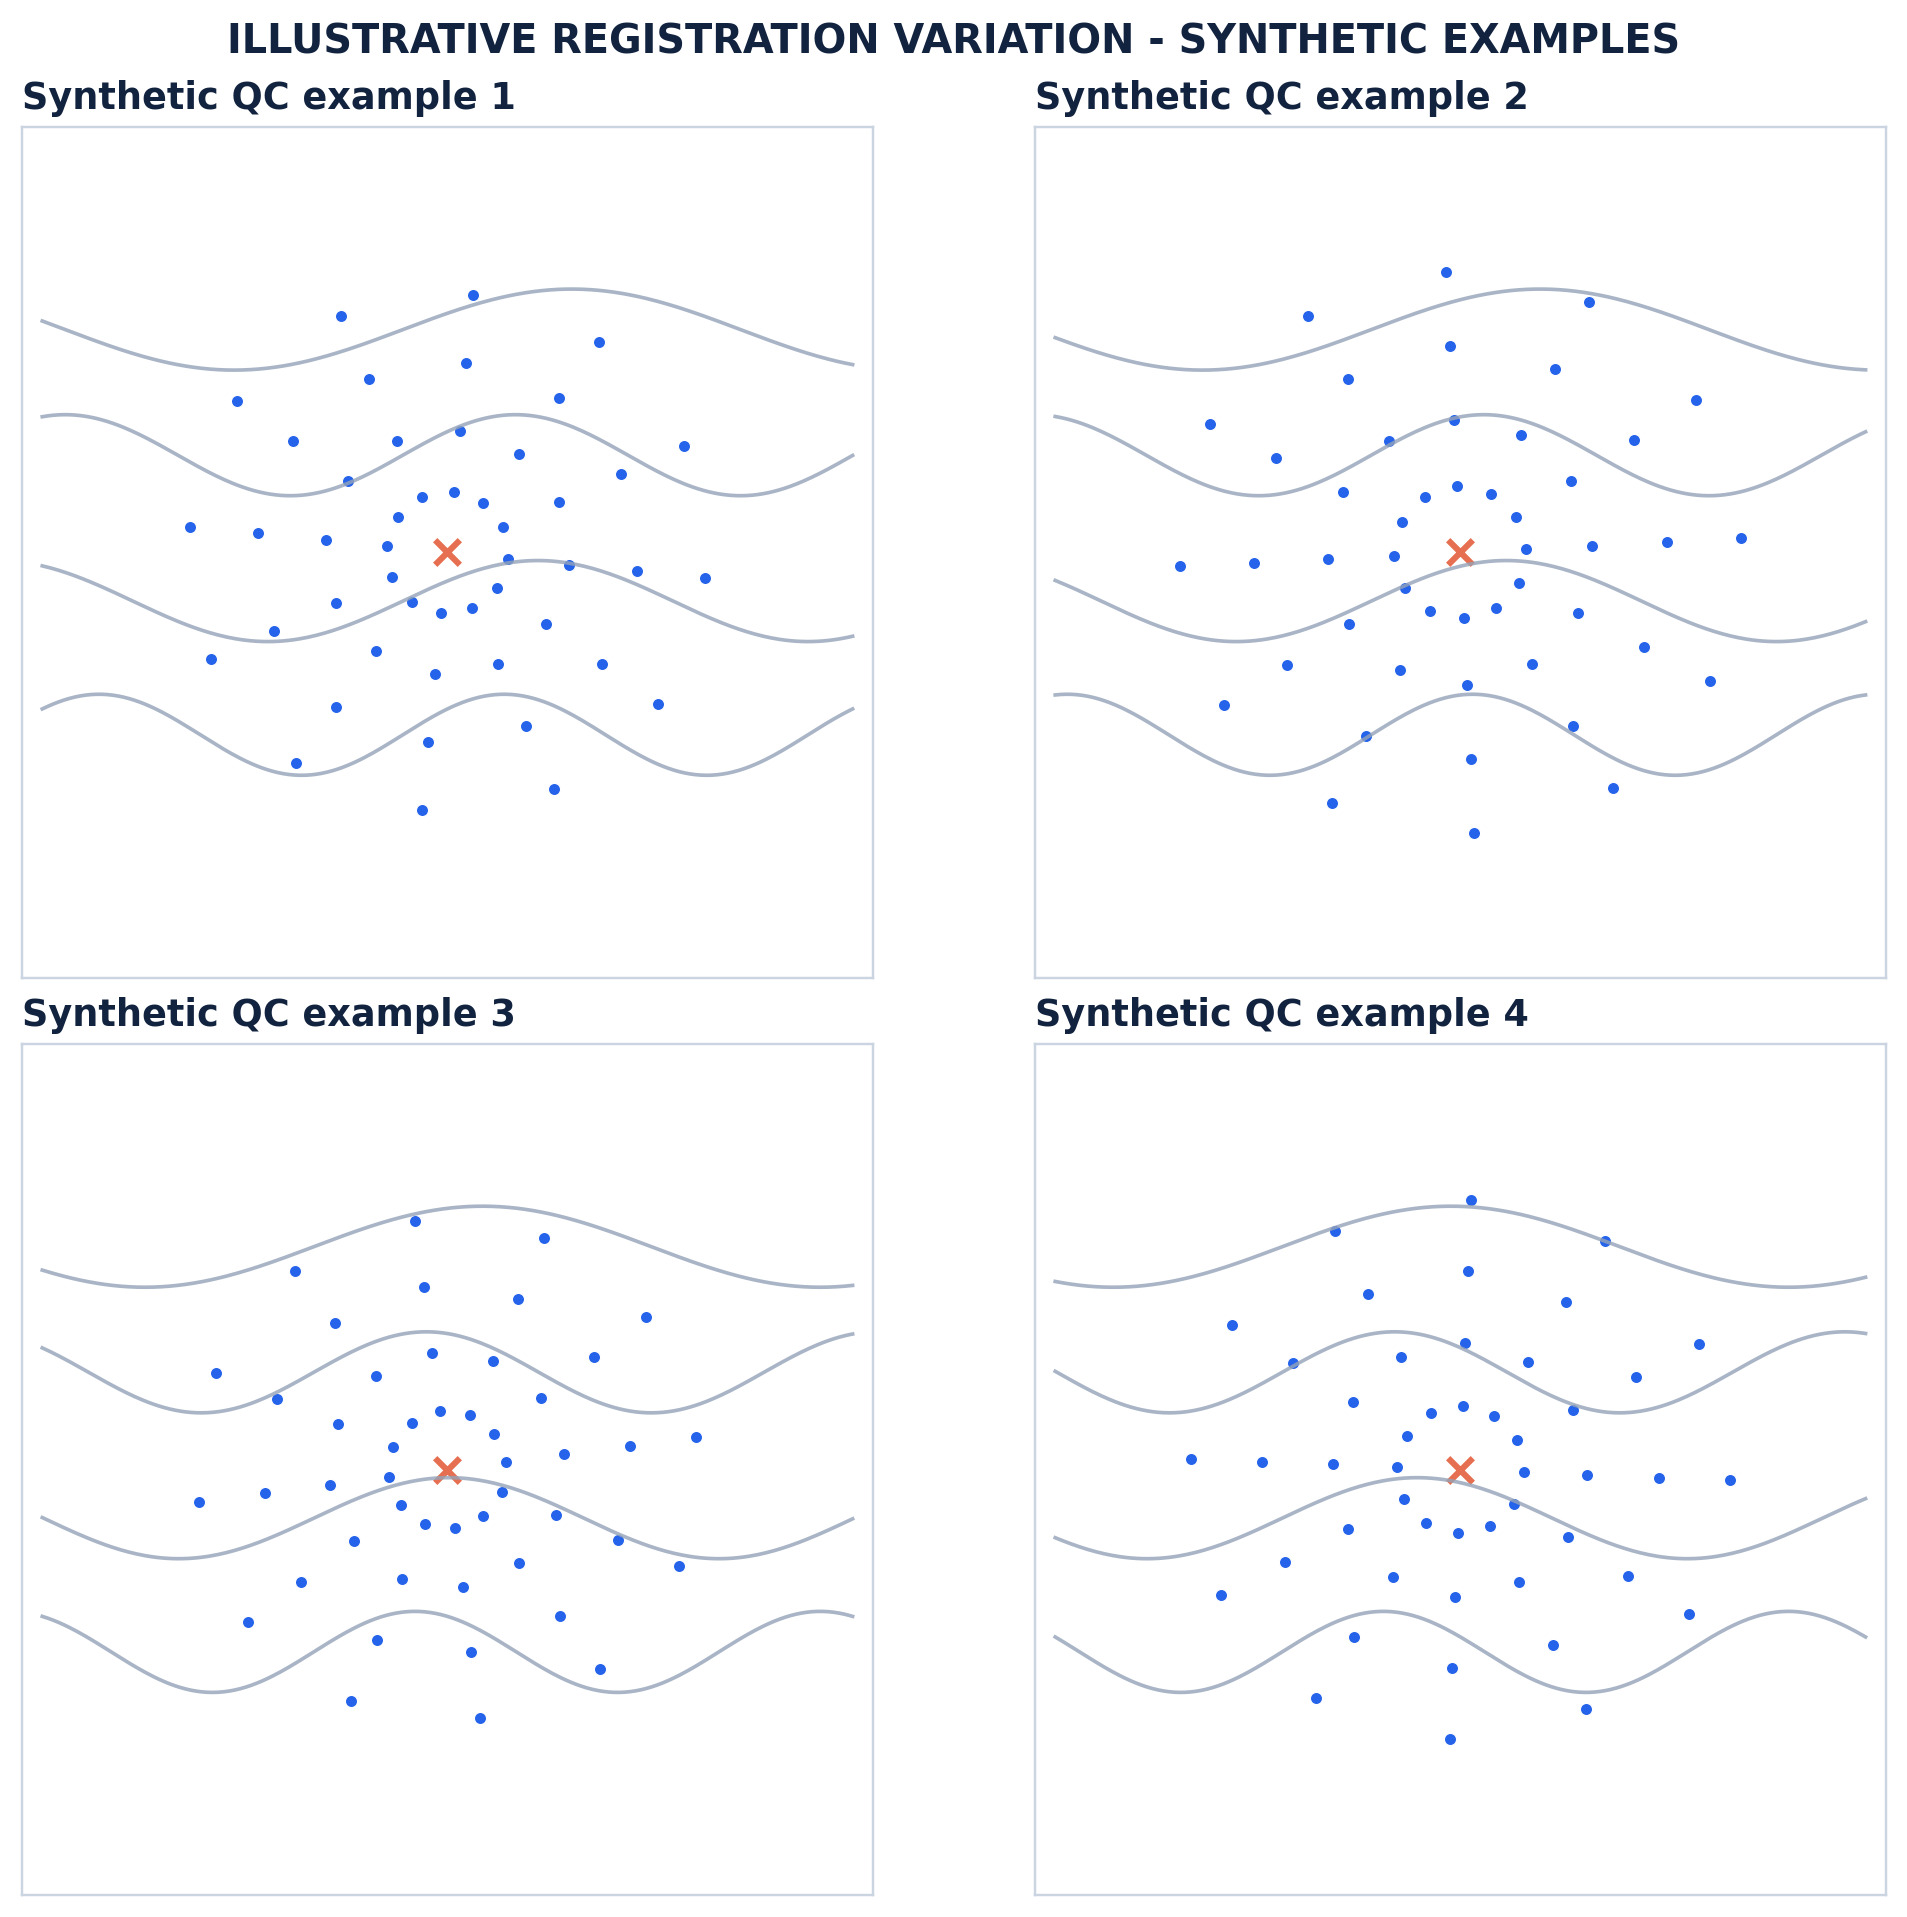
\includegraphics[width=0.92\textwidth]{figure_supplementary_qc_public.png}
  \caption{Supplementary registration schematics using synthetic coordinates and abstract geometric curves.}
  \label{fig:supplementary-qc}
\end{figure}


\clearpage
\renewcommand{\bibname}{References}
\phantomsection
\addcontentsline{toc}{chapter}{References}
\bibliographystyle{unsrtnat}
\bibliography{references}

\end{document}
